\documentclass[12pt]{beamer}

%%%%%%%%%%%%%%%%%%% Theme

\usetheme{metropolis}

%%%%%%%%%%%%%%%%%%% Packages

\usepackage[french, english]{babel}
\usepackage{packages/sleek-beamer}

%%%%%%%%%%%%%%%%%%% Bibliography

\addbibresource{./resources/bib/references.bib}

%%%%%%%%%%%%%%%%%%% Titlepage

\title{Renewable Energy Production Forecast}
\subtitle{PROJ0016 - Big Data Project}
\author{Yann Claes, Gaspard Lambrechts and François Rozet}
\institute{University of Liège}
\date{\today}
\titlelogo{./resources/pdf/logo.pdf}
\framelogo{./resources/pdf/logo.pdf}

%%%%%%%%%%%%%%%%%%%

\DeclareSIUnit\voltampere{VA}

\makeatletter
\def\blfootnote{\gdef\@thefnmark{}\@footnotetext}
\makeatother

%%%%%%%%%%%%%%%%%%%

\begin{document}

\maketitle

\begin{frame}[standout]
    \vspace{1em}
    \begin{quote}
        \emph{\enquote{How much renewable energy will be produced tomorrow in Liège ?}}
    \end{quote}
\end{frame}

\begin{frame}{Approach}
    We divided our approach in three branches :
    \begin{enumerate}
        \item Assessing the number and location of photovoltaic units;
        \item Estimating the photovoltaic energy production;
        \item Estimating the wind energy production.
    \end{enumerate}
    \begin{figure}
        \centering
        \vspace{-1em}
        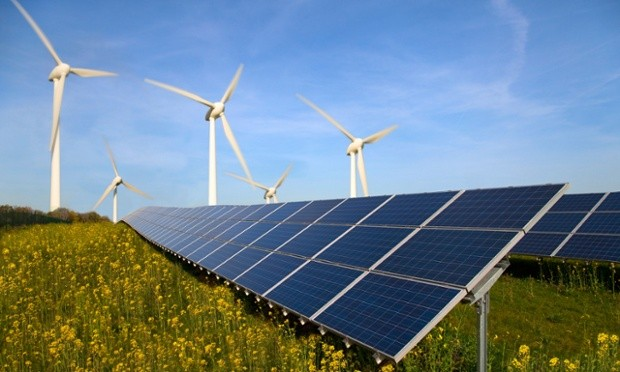
\includegraphics[height=0.4\textheight]{resources/jpg/temp.jpeg}
        \vspace{-1em}
    \end{figure}
\end{frame}

\section{Photovoltaic panels mapping}

\begin{frame}{Approach}
    We couldn't find appropriate records of photovoltaic installations in Liège.
    
    We decided to \emph{estimate} the number and location of photovoltaic panels using \alert{remote sensing}, in particular using \alert{aerial} or \alert{satellite} imagery.
\end{frame}

\begin{frame}{Wallonia aerial images}
    Wallonia possesses a geographic information website \alert{WalOnMap}. It uses the \alert{Web Map Tiles Service} standard.
    
    Using \alert{\texttt{owslib}} Python library we could retrieve these tiles ($512 \times 512$ images).
    
    Unfortunately, the images have a quite \alert{low quality}.
\end{frame}

\begin{frame}{Detection model -- U-Net}
    We decided to use a tweaked version of \alert{U-Net} \parencite{ronneberger2015u}, a well known segmentation network.
    
    We implemented it and trained it using the \alert{\texttt{PyTorch}} Python library.
    
    \blfootnote{This part of the project was conducted in parallel with our project of \emph{Deep Learning}. Therefore, we won’t explain the implementation and training process (algorithm, loss function, etc.) in this presentation.}
\end{frame}

\begin{frame}{Training set}
    We found a dataset \parencite{bradbury2016distributed} of over \num{19 000} solar panels across \num{601} high resolution ($5000 \times 5000$) images from four cities in California.
    
    Using the coordinates (provided as polygon vertices), we produced \alert{segmentation masks} in order to train our model.
\end{frame}

\begin{frame}
    \begin{figure}
        \centering
        \vspace{1em}
        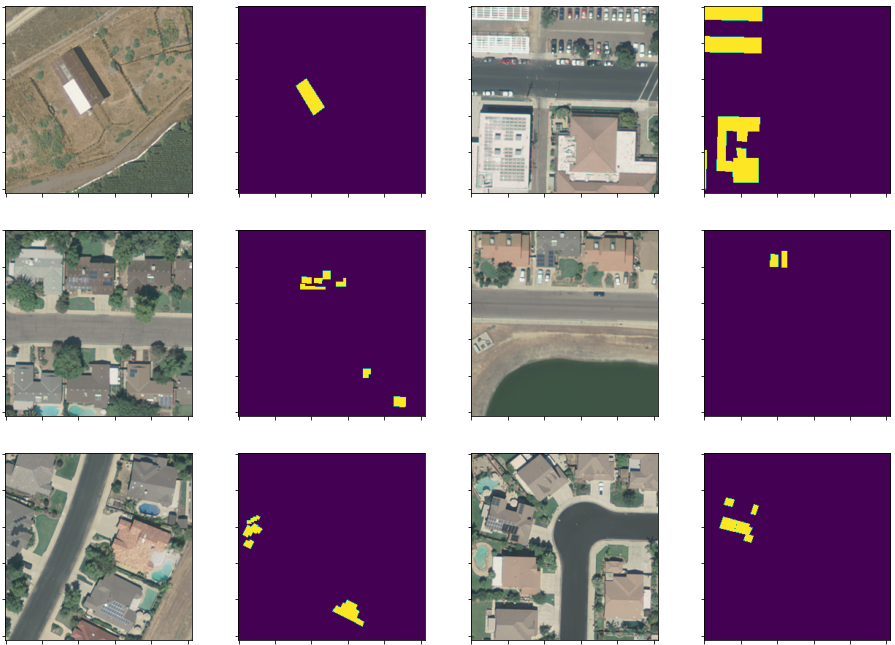
\includegraphics[width=\textwidth]{resources/png/masks.png}
        \vspace{-2em}
        \noskipcaption{Training set images sample with their masks.}
    \end{figure}
\end{frame}

\begin{frame}{Data augmentation}
    The training images are very different (\alert{colorimetry}, \alert{blurriness}, etc.) from the images of \alert{WalOnMap}.
    
    We decided to \alert{augment} our training set. Our approach is to randomly apply transformations to the images \emph{while training}.
    
    Transformations : rotations, flips, brightness, contrast, smoothing, sharpening, etc.
\end{frame}

\begin{frame}
    \begin{figure}
        \centering
        \vspace{1em}
        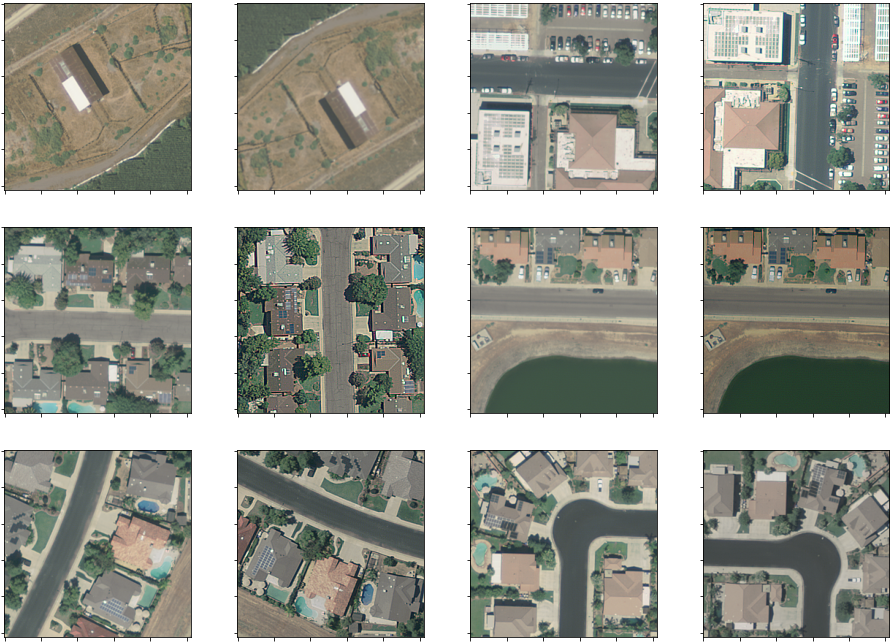
\includegraphics[width=\textwidth]{resources/png/augmentation.png}
        \vspace{-2em}
        \noskipcaption{Training set augmentation sample.}
    \end{figure}
\end{frame}

\begin{frame}{Results -- California}
    \begin{figure}
        \centering
        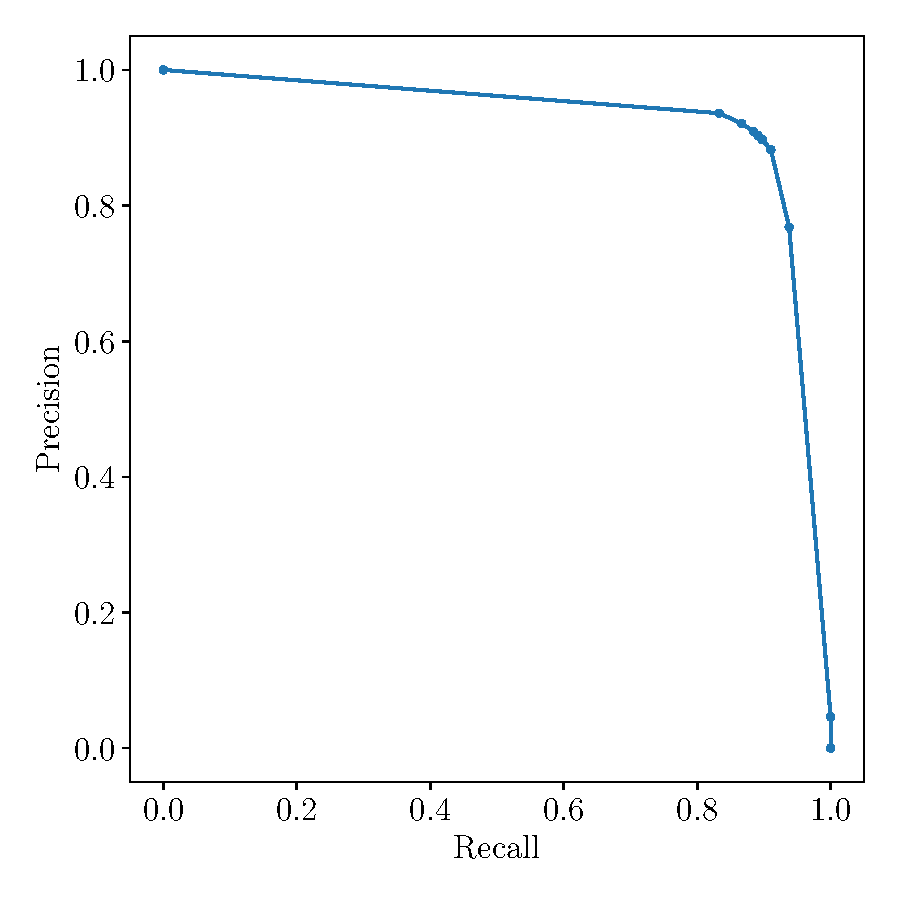
\includegraphics[height=0.8\textheight]{resources/pdf/precision_recall.pdf}
        \vspace{-1em}
        \noskipcaption{Precision-recall curve on the Californian test set.}
    \end{figure}
\end{frame}

\begin{frame}{Californian results}
    Our model :
    \begin{align*}
        \text{average precision} & = \SI{92.51}{\percent} \\
        \text{precision}(0.5) & = \SI{90.3}{\percent} \\
        \text{recall}(0.5) & = \SI{89.1}{\percent}
    \end{align*}
    
    \visible<2>{
    \textcite{malof2016deep} :
    \begin{align*}
        \text{precision}(?) & = \SI{80}{\percent} \\
        \text{recall}(?) & = \SI{72}{\percent}
    \end{align*}
    }
\end{frame}

\begin{frame}{Fine tuning}
    However, the results on \alert{WalOnMap} were not satisfactory.
    
    Therefore, we \alert{fine-tuned} our model for a few more epochs on \num{550} \alert{WalOnMap} images we \alert{hand-annotated}.
    
    \blfootnote{111 other images are kept for metric evaluation.}
\end{frame}

\begin{frame}{Fine tuning}
    \begin{figure}
        \centering
        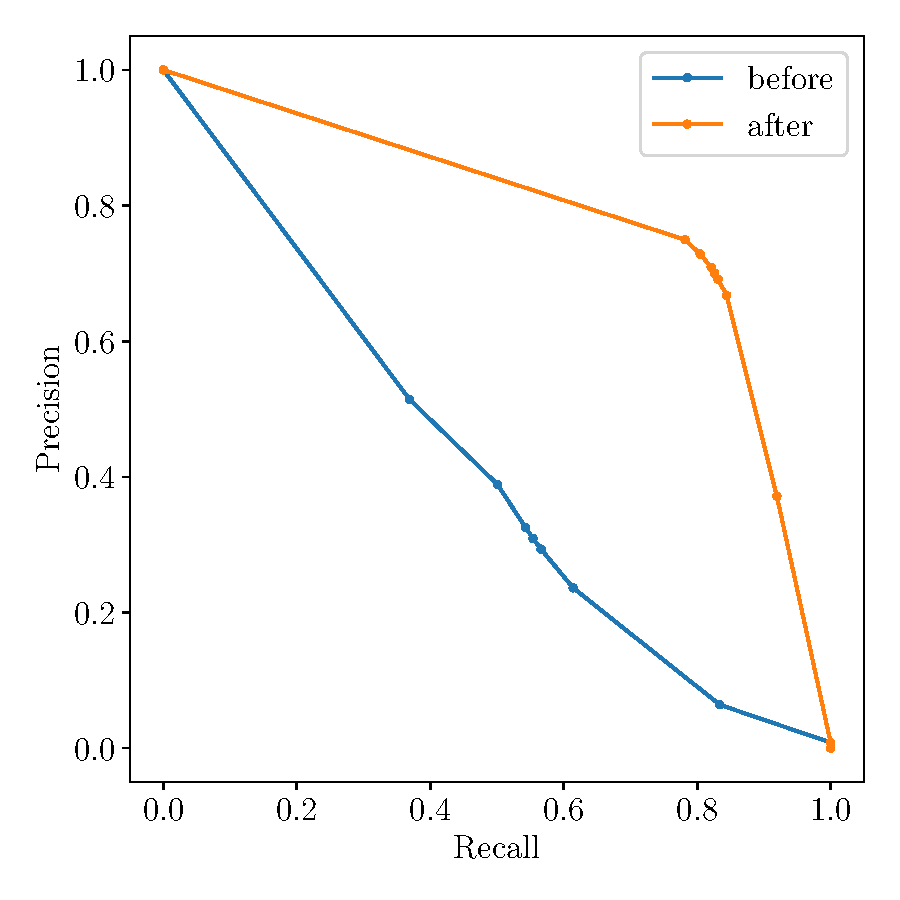
\includegraphics[height=0.8\textheight]{resources/pdf/before_after.pdf}
        \vspace{-1em}
        \noskipcaption{Precision-recall curve before and after fine-tuning.}
    \end{figure}
\end{frame}

\begin{frame}{Fine tuning}
    \begin{align*}
        \text{average precision} & = \SI{78.3}{\percent} \\
        \text{precision}(0.5) & = \SI{71.3}{\percent} \\
        \text{recall}(0.5) & = \SI{82.6}{\percent}
    \end{align*}
\end{frame}

\begin{frame}{Mapping}
    Finally, we applied our fine-tuned model on the \alert{\num{846703}} tiles of the \alert{Province of Liège}. After \alert{\SI{1.5}{\day}} we obtained the location and shape (polygons) of \alert{\num{64463}} PV installations covering \alert{\SI{2554505}{\meter\squared}} of land.
\end{frame}

\begin{frame}
    \begin{figure}
        \centering
        \vspace{1em}
    	\begin{subfigure}{0.48\textwidth}
    		\centering
    		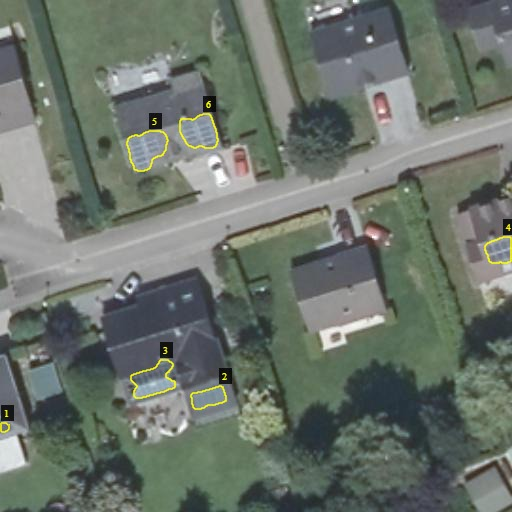
\includegraphics[width=\textwidth]{resources/jpg/609483_533144.jpg}
    	\end{subfigure}
    	\hspace{0em}
    	\begin{subfigure}{0.48\textwidth}
    		\centering
    		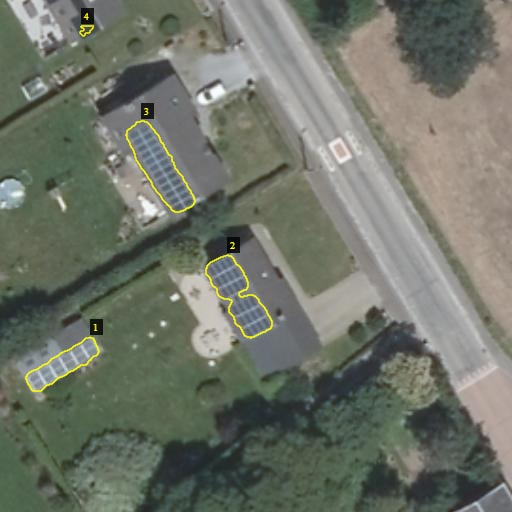
\includegraphics[width=\textwidth]{resources/jpg/609525_533266.jpg}
    	\end{subfigure}
    \end{figure}
\end{frame}

\begin{frame}
    \begin{figure}
        \centering
        \vspace{1em}
    	\begin{subfigure}{0.48\textwidth}
    		\centering
    		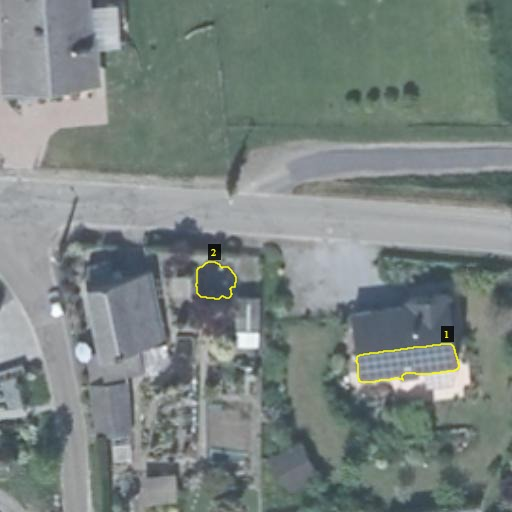
\includegraphics[width=\textwidth]{resources/jpg/609591_532657.jpg}
    	\end{subfigure}
    	\hspace{0em}
    	\begin{subfigure}{0.48\textwidth}
    		\centering
    		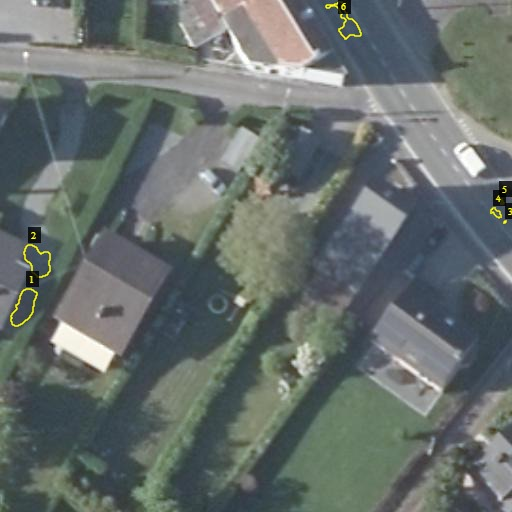
\includegraphics[width=\textwidth]{resources/jpg/609601_533193.jpg}
    	\end{subfigure}
    \end{figure}
\end{frame}

\begin{frame}{Binding}
    As such, the locations and shapes are not usable for the power production model. Therefore, we summarized each detected installation into \alert{3 quantities} :
    \begin{itemize}
        \item its geospatial location (latitude and longitude);
        \item its surface;
        \item its azimuth angle.
    \end{itemize}
\end{frame}

\section{Photovoltaic production}
\begin{frame}{Approach}
    As specified by the guidelines, we opted for a \alert{short-term} prediction task.
    
    3 possibilities (\cite{nespoli2019day}):
    \begin{itemize}
        \item Statistical methods: regression, artificial neural networks
        \item Physical methods
        \item Hybrid methods: mix of statistical and physical
    \end{itemize}
\end{frame}

\begin{frame}{Approach}
    As specified by the guidelines, we opted for a \alert{short-term} prediction task.
    
    3 possibilities:
    \begin{itemize}
        \item Statistical methods: regression, artificial neural networks
        \item \alert{Physical methods}
        \item Hybrid methods: mix of statistical and physical
    \end{itemize}

    Our main idea was to rely on physical \alert{intuition}.
    
    $\Rightarrow$ Build \alert{simple} physical models.
\end{frame}

\begin{frame}{Approach}
    Build a \emph{panelwise} model that we would scale up $\Rightarrow$ focus on a \alert{small} scale first (ULiège) and assess the obtained results.
    
    Need panels characteristics:
    \begin{itemize}
        \item Location (latitude - longitude)
        \item Area
        \item Surface azimuth
    \end{itemize}
    
    Build a second model, relying on available solar data:
    \begin{itemize}
        \item Installed power
        \item Peak area
    \end{itemize}
\end{frame}

\begin{frame}{Collecting data}
    We needed 2 types of data:
    \begin{itemize}
        \item Photovoltaic \alert{production} data
        \item \alert{Irradiance} data
    \end{itemize}
\end{frame}

\begin{frame}{Collecting data}
    We obtained production and irradiance data for ULiège 
    
    $\Rightarrow$ \alert{evaluate} our panelwise model.
    
    We needed the same, at a \alert{larger scale}. Only \alert{publicly available} production data: Elia (measurements, forecasts, etc.), with a granularity of 15 minutes.
\end{frame}

\begin{frame}{Collecting data}
    However, Elia provides photovoltaic production data at a \alert{provincial} scale.
    
    Hence, to get reference data to \alert{compare} to, we opted for predicting the photovoltaic production of the province of Liège. 

    As far as irradiance data is concerned, we discovered \alert{Solcast}'s API (historical and forecast data). It provides data at a granularity of 30 minutes.
\end{frame}

\begin{frame}{Pre-processing data}
    To match the irradiance granularity, we simply \alert{averaged} Elia's measures for each 30-minutes period.
    
    Dealing with missing data was done using \alert{linear interpolation}.
\end{frame}

\begin{frame}{Panelwise model}
    Our panelwise model relies on the computation of two main \alert{solar angles}:
    \begin{itemize}
        \item Incidence angle $\theta$ between the sun rays and the normal vector of the panel installation (depends on other solar angles)
        \item Solar altitude $alt$
    \end{itemize}
    The cosine of $\theta$ relies on:
    \begin{itemize}
        \item Surface azimuth
        \item Declination angle $\delta$
        \item Latitude and longitude
        \item Hour angle $\omega$
        \item Tilt angle $\beta$
    \end{itemize}
\end{frame}

\begin{frame}{Panelwise model}
    We derived the following model
    \begin{equation*}
        P = \frac{\eta I \cos(\theta) A}{\sin(alt)} \quad [\si{\watt}]
    \end{equation*}
\end{frame}

\begin{frame}{Panelwise model}
    \begin{figure}
        \centering
        \begin{subfigure}{0.48\textwidth}
        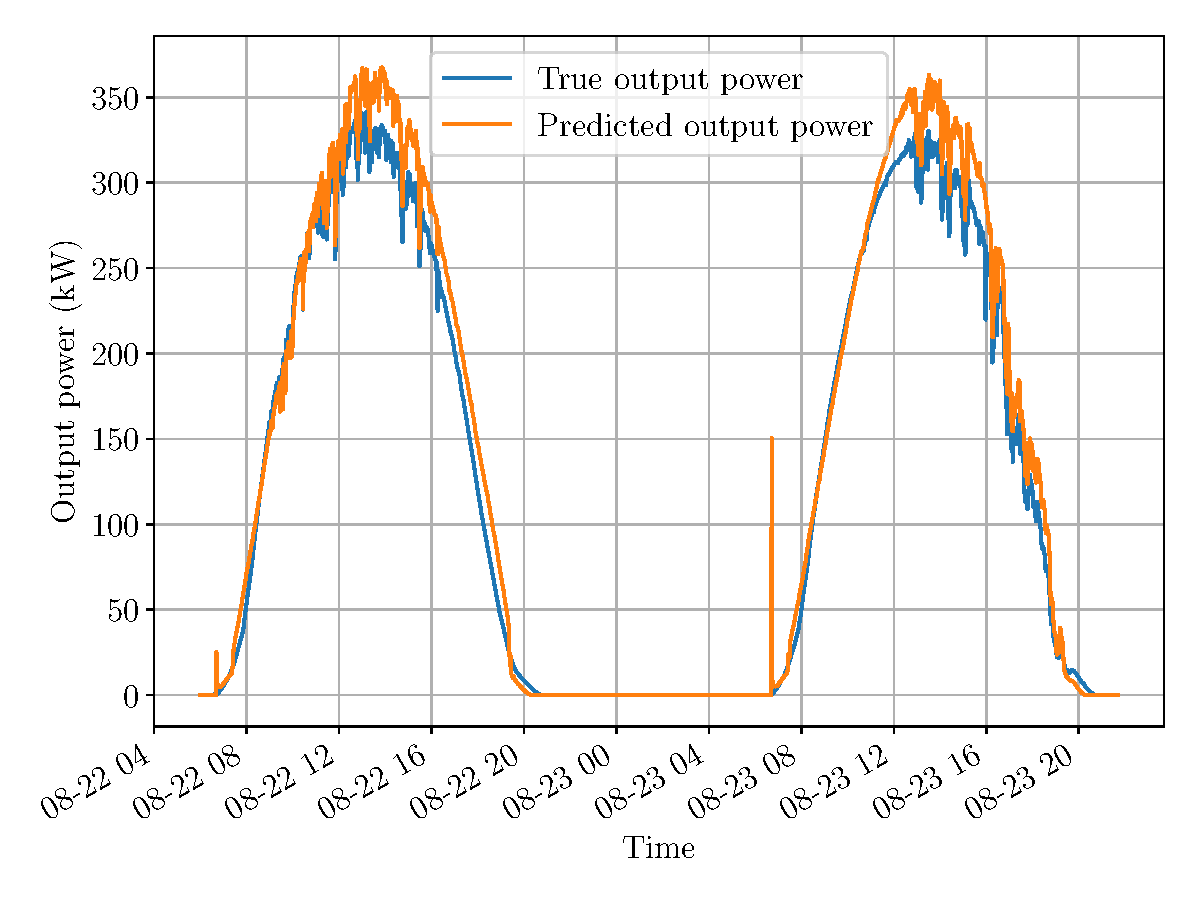
\includegraphics[width=\textwidth]{resources/pdf/sart_tilman_22-08-2019.pdf}
        \end{subfigure}
        \hspace{0em}
        \begin{subfigure}{0.48\textwidth}
        \centering
        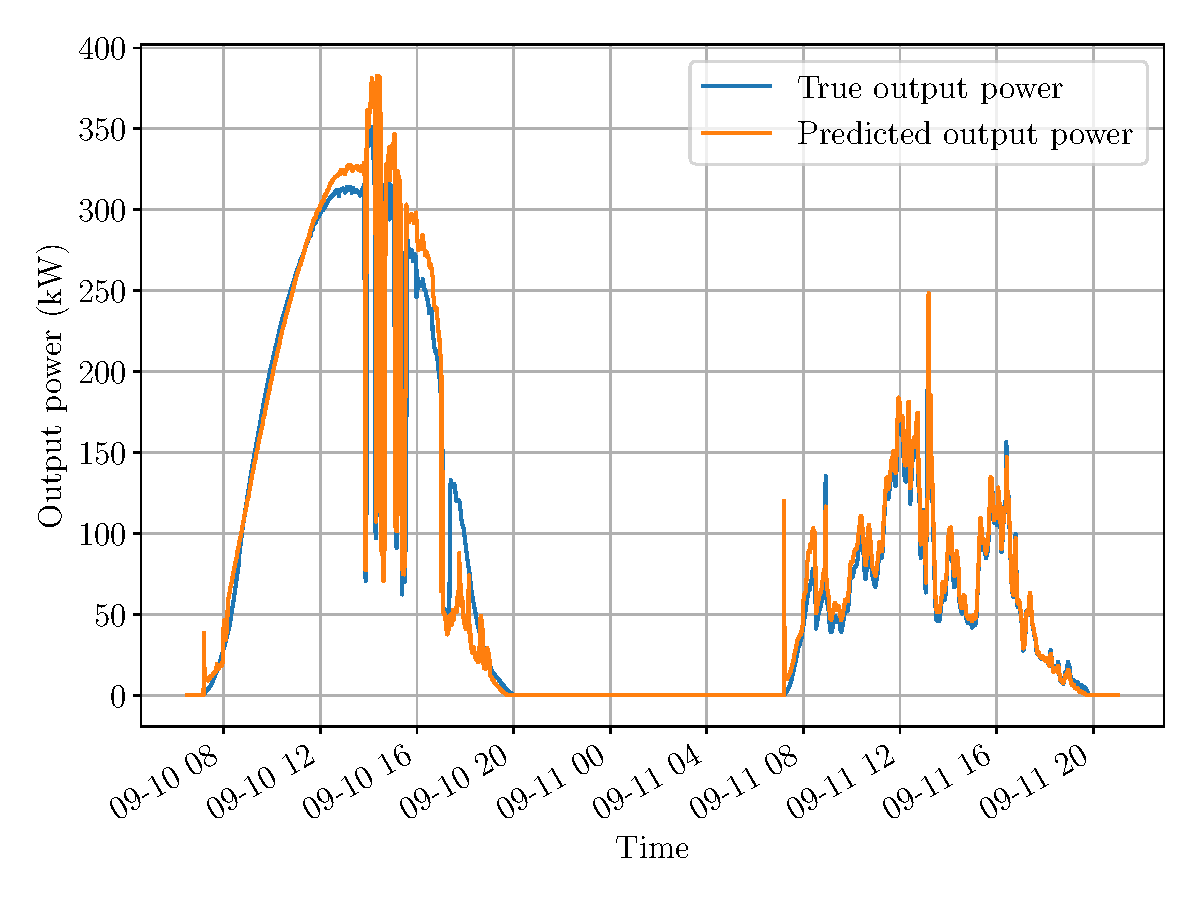
\includegraphics[width=\textwidth]{resources/pdf/sart_tilman_10-09-2019.pdf}
        \end{subfigure}
    \end{figure}
\end{frame}

\begin{frame}{Panelwise model}
    With \alert{fixed} parameters ($\eta$, $\beta$), our model is very rigid and dependent on the quality of our \alert{panels mapping} and on the irradiance \alert{forecasts}.
    
    $\Rightarrow$ introduce uncertainties.
\end{frame}

\begin{frame}{Panelwise model}
    We considered the quantity
    \begin{equation*}
        naive\_power = \frac{I \cos(\theta) A}{\sin(alt)}
    \end{equation*}
    as fixed and modeled uncertainties on $\eta$, using \alert{PyStan} as probabilistic programming language.
    
    To model the \alert{posterior} distribution of $\eta$, we \emph{fit} using Elia's production measurements over the past 7 days.
\end{frame}

\begin{frame}{Panelwise model}
    The predicted photovoltaic power is modeled with a \alert{normal} distribution centered around
    \begin{equation*}
        \eta \times forecast\_power
    \end{equation*}
    where $forecast\_power$ is computed using irradiance \alert{forecasts}, and $\eta$ is drawn from its posterior distribution.
    
    \blfootnote{Results will be shown later.}
\end{frame}

\begin{frame}{Provincial model}
    We decided to call our \alert{second} model the \emph{provincial} model, although both will be used at a provincial scale.
    
    Here, we model our photovoltaic production using solar data, such as:
    \begin{itemize}
        \item Installed power in the province of Liège
        \item Estimate of the peak area
    \end{itemize}
\end{frame}

\begin{frame}{Provincial model}
    We derived the following model
    \begin{equation*}
        P = \eta I A \quad [\si{\watt}]
    \end{equation*}
    where $\eta$ is the panel efficiency, $I$ is the irradiance and $A = peak\_area \times \si{\kilo\voltampere}$ is the area of panels in the province (with \si{\kilo\voltampere} being the installed power).
\end{frame}

\begin{frame}{Provincial model}
    Similarly to the panelwise model, we also modeled \alert{uncertainties} to make the model more flexible.
    
    Again, each \alert{posterior} is built using Elia's production measurements over the past 7 days, and the predicted power is modeled with a normal distribution.
\end{frame}

\begin{frame}{Analysis of both models}
    To evaluate the quality of both models, we applied the following \alert{procedure}: for a given day of prediction, we construct both posterior models using Elia's production measurements over the past 7 days and predict for the considered day.
    
    We \alert{compare} the predictions of our models with respect to Elia's measurements, using the MSE and RMSE. Beforehand, we \alert{remove} night observations to only evaluate when there is a nonzero produced power.
\end{frame}

\begin{frame}{Analysis of both models}
    We will compare our posterior models with their prior (rigid) counterparts, along with two simple \alert{baselines}:
    \begin{itemize}
        \item Predict for day $D$ the measured production of day $D - 1$
        \item Predict for day $D$ the average measured production over the last 7 days.
    \end{itemize}
    
    To get \alert{representative} results, we conducted the procedure on the whole 2019 year (using irradiance measures since past irradiances forecasts were not available). 
\end{frame}

\begin{frame}{Results}
    \begin{table}[H]
\centering
\begin{tabular}{l|c|c}
                           & MSE     & RMSE
                           \\ \hline
Prior panelwise model      & 2852.73 & 49.25 $\pm$ 20.68
\\\hline
\alert{Posterior panelwise model}  & 510.84  & 20.06 $\pm$ 10.42 \\ \hline
Prior provincial model     & 608.98  & 21.94 $\pm$ 11.31 \\ \hline
\alert{Posterior provincial model} & 431.23  & 18.49 $\pm$ 9.46  \\ \hline
Baseline 1                 & 2195.60 & 38.87 $\pm$ 26.19 \\ \hline
Baseline 2                 & 1816.74 & 37.34 $\pm$ 20.56 \\ \hline
\alert{Elia's forecast}            & 381.85  & 16.79 $\pm$ 10.01
\end{tabular}
\caption{Mean MSE and mean RMSE, along with standard deviation, for 2019 (using irradiance measurements), in \si{\mega\watt}.}
\end{table}
\end{frame}

\begin{frame}{Analysis of both models}
    To get more \emph{real-life} representative results, we conducted the same procedure considering April 2020. This time, we use irradiance \alert{forecasts}.
\end{frame}

\begin{frame}{Results}
    \begin{table}[]
\centering
\begin{tabular}{l|c|c}
                           & MSE     & RMSE              \\ \hline
Prior panelwise model      & 5316.57 & 62.85 $\pm$ 37.66 \\ \hline
\alert{Posterior panelwise model}  & 1563.30 & 32.23 $\pm$ 23.33 \\ \hline
Prior provincial model     & 2210.83 & 42.44 $\pm$ 20.62 \\ \hline
\alert{Posterior provincial model} & 1595.59 & 32.63 $\pm$ 23.48 \\ \hline
Baseline 1                 & 2616.99 & 36.34 $\pm$ 36.68 \\ \hline
Baseline 2                 & 2339.52 & 40.87 $\pm$ 26.34 \\ \hline
\alert{Elia's forecast}            & 324.85  & 15.16 $\pm$ 10.11
\end{tabular}
\caption{Mean MSE and mean RMSE along with standard deviation, for April 2020 (using irradiance forecasts), in \si{\mega\watt}.}
\end{table}
\end{frame}

\begin{frame}{Results}
    \begin{figure}[H]
	\centering
	\begin{subfigure}{0.48\textwidth}
		\centering
		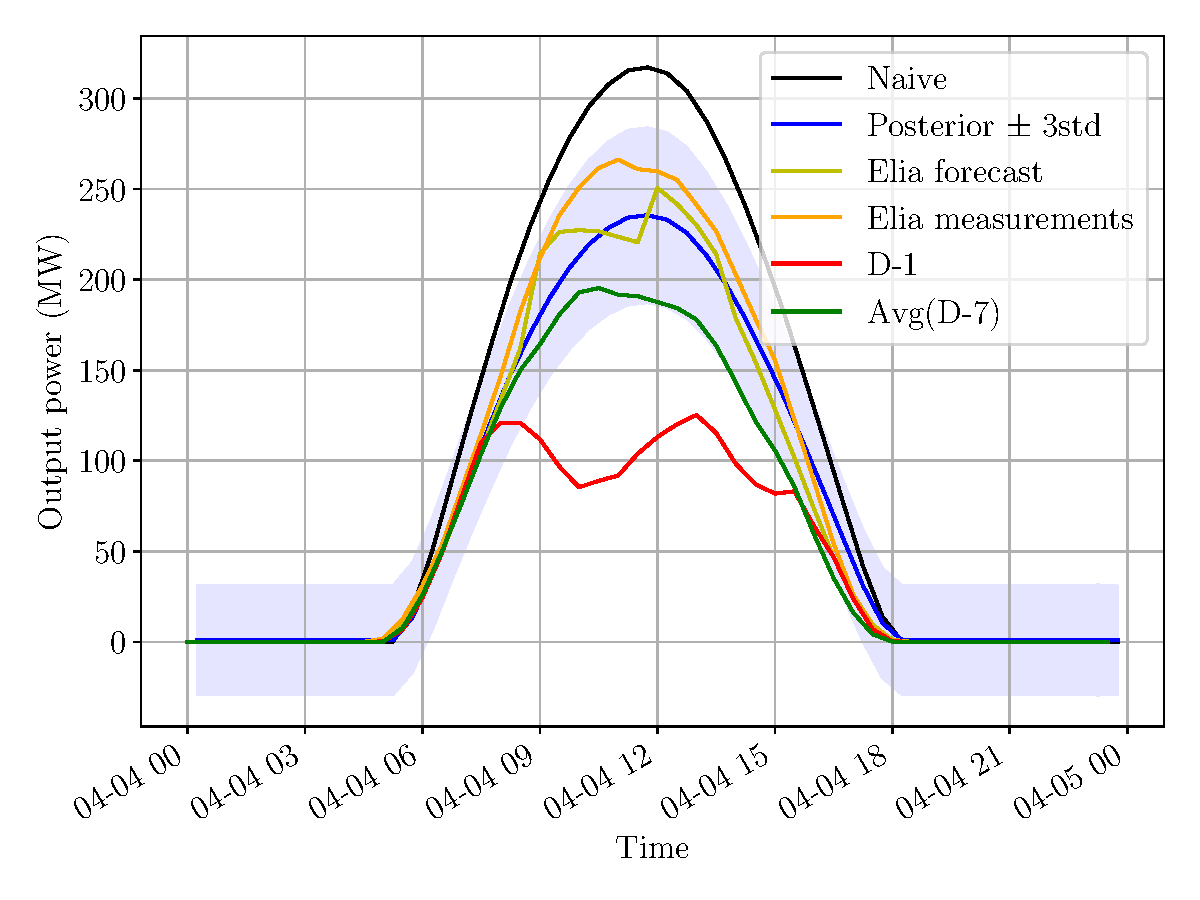
\includegraphics[width=\textwidth]{resources/pdf/solar_panelwise_START_FOR_04-04-2020.pdf}
		\noskipcaption{Panelwise model (using irradiance forecasts).}
	\end{subfigure}
	\hspace{0em}
	\begin{subfigure}{0.48\textwidth}
		\centering
		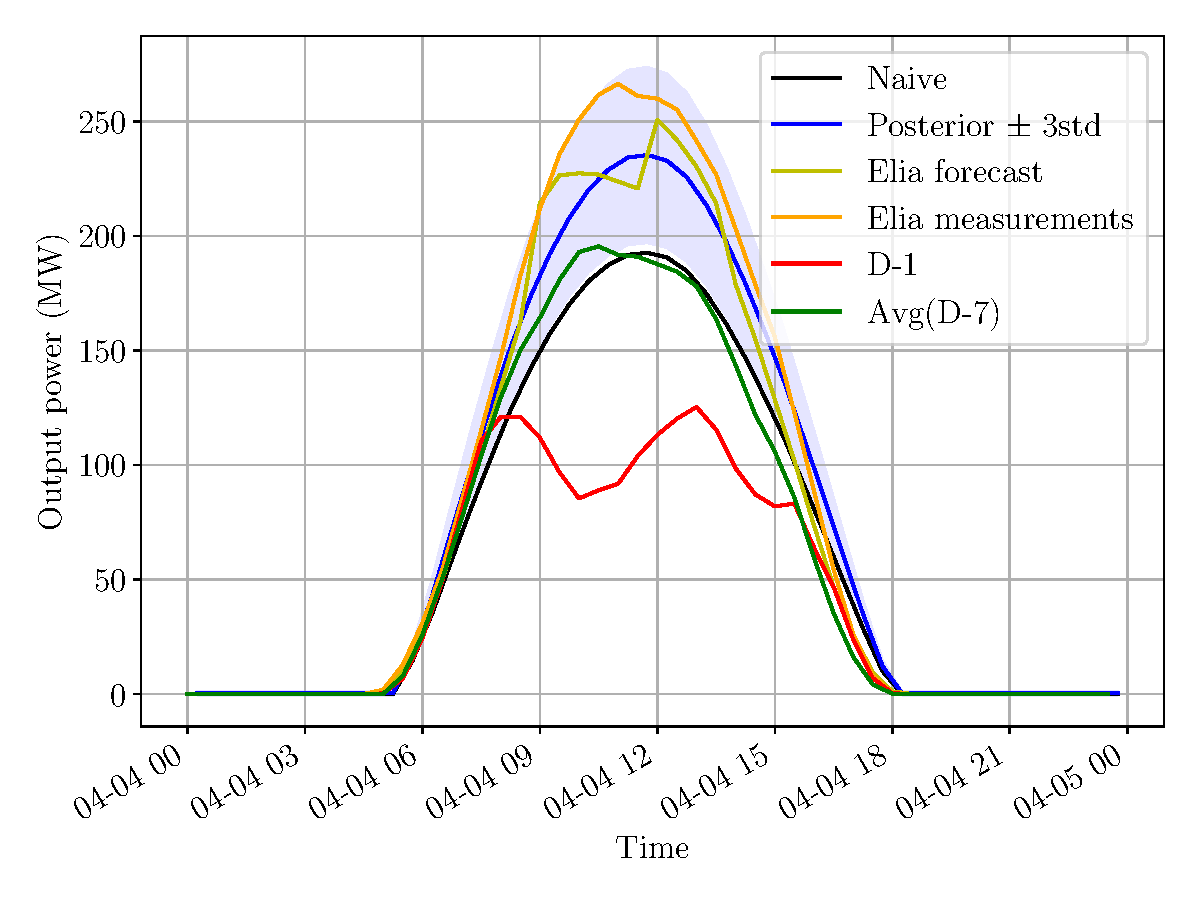
\includegraphics[width=\textwidth]{resources/pdf/solar_provincial_START_FOR_04-04-2020.pdf}
		\noskipcaption{Provincial model (using irradiance forecasts).}
	\end{subfigure}
\end{figure}
\end{frame}

\begin{frame}{Results}
    \begin{figure}[H]
	\centering
	\begin{subfigure}{0.48\textwidth}
		\centering
		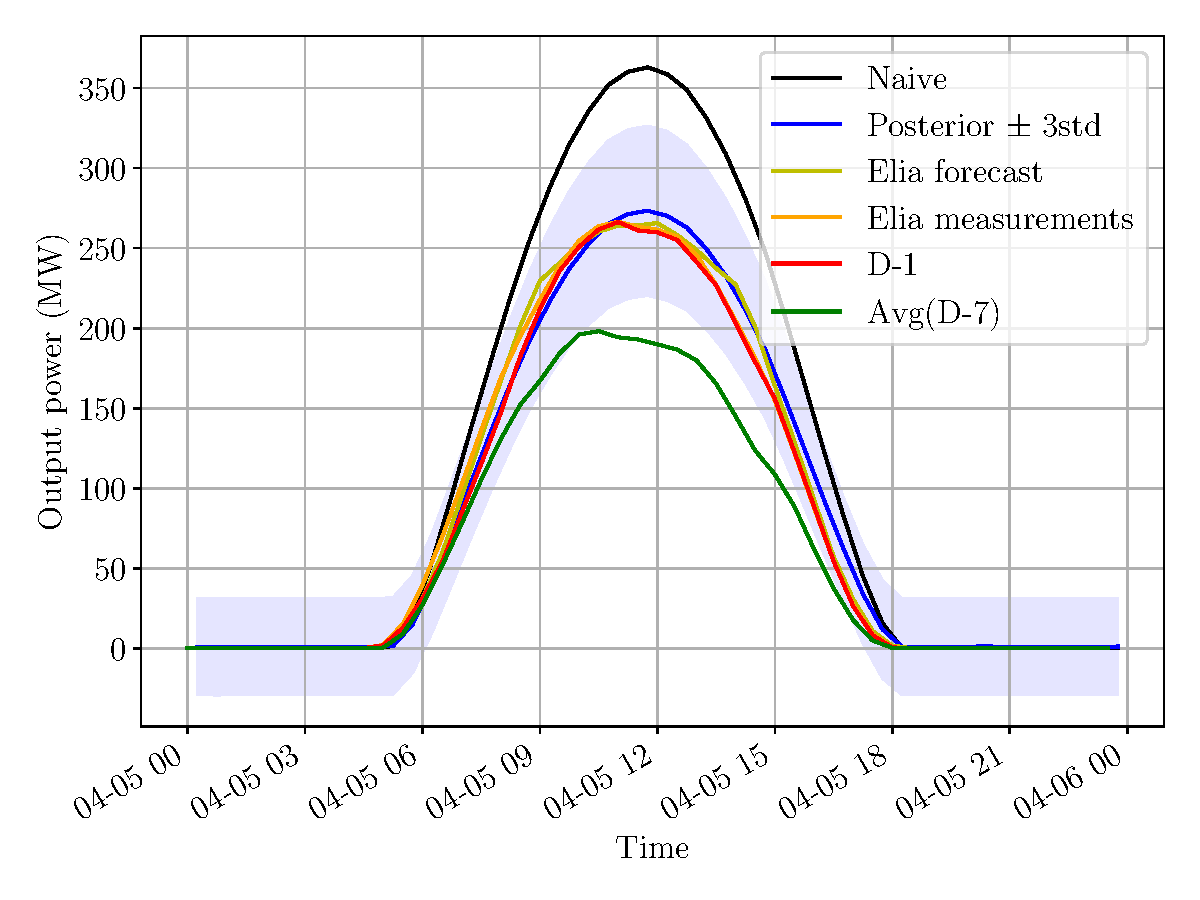
\includegraphics[width=\textwidth]{resources/pdf/solar_panelwise_START_FOR_05-04-2020.pdf}
		\caption{Panelwise model (using irradiance forecasts).}
	\end{subfigure}
	\hspace{0em}
	\begin{subfigure}{0.48\textwidth}
		\centering
		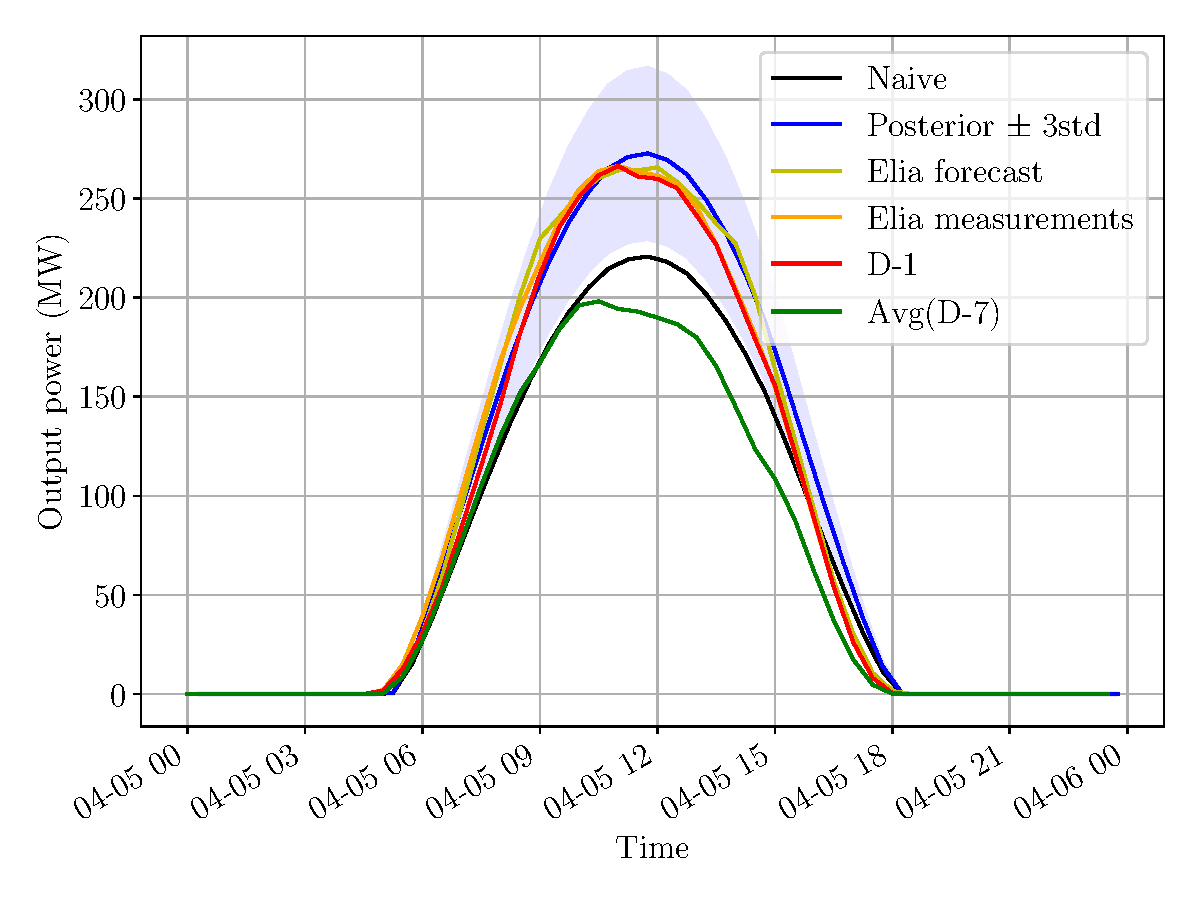
\includegraphics[width=\textwidth]{resources/pdf/solar_provincial_START_FOR_05-04-2020.pdf}
		\noskipcaption{Provincial model (using irradiance forecasts).}
	\end{subfigure}
\end{figure}
\end{frame}


\begin{frame}{Results}
    \begin{figure}[H]
	\centering
	\begin{subfigure}{0.48\textwidth}
		\centering
		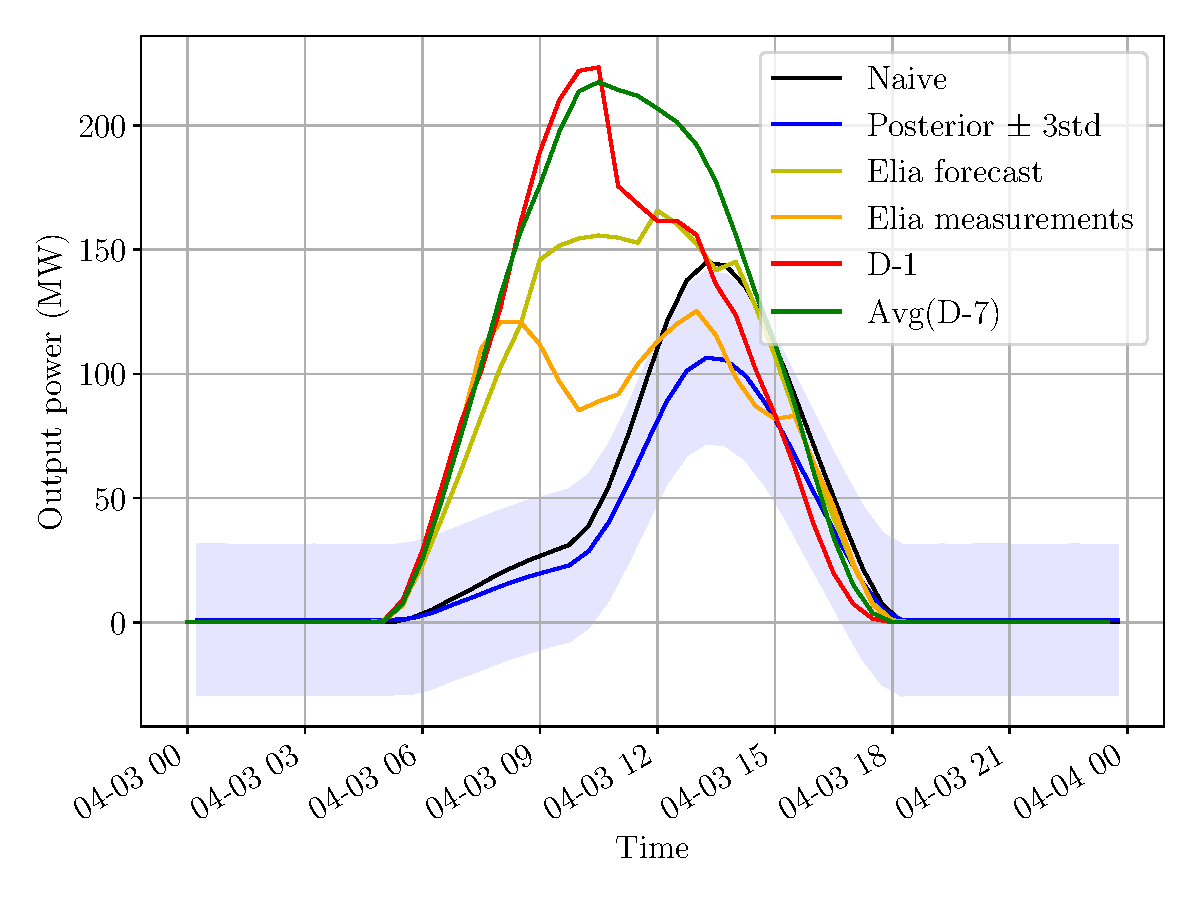
\includegraphics[width=\textwidth]{resources/pdf/solar_panelwise_START_FOR_03-04-2020.pdf}
		\noskipcaption{Panelwise model (using irradiance forecasts).}
	\end{subfigure}
	\hspace{0em}
	\begin{subfigure}{0.48\textwidth}
		\centering
		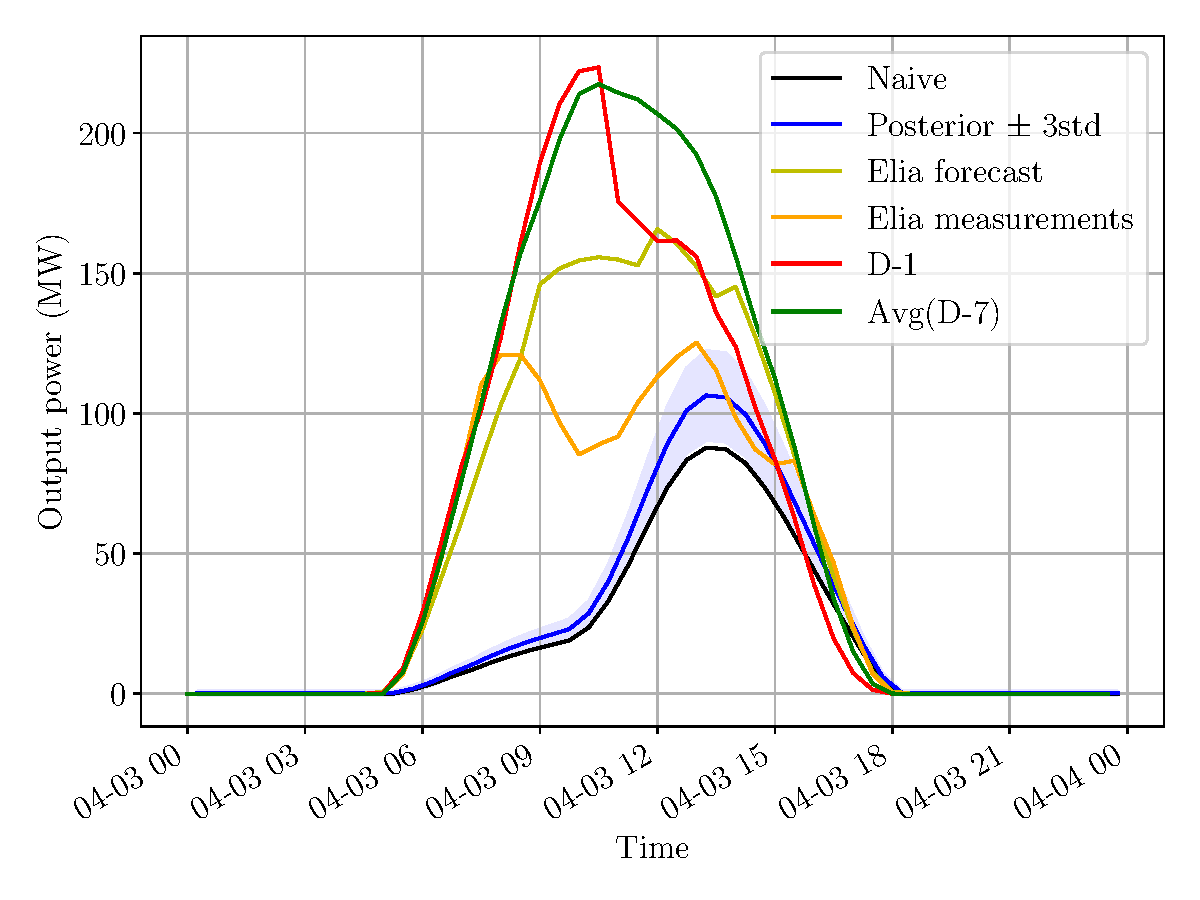
\includegraphics[width=\textwidth]{resources/pdf/solar_provincial_START_FOR_03-04-2020.pdf}
		\noskipcaption{Provincial model (using irradiance forecasts).}
	\end{subfigure}
\end{figure}
\end{frame}

\begin{frame}{Results}
    \begin{figure}[H]
	\centering
	\begin{subfigure}{0.48\textwidth}
		\centering
		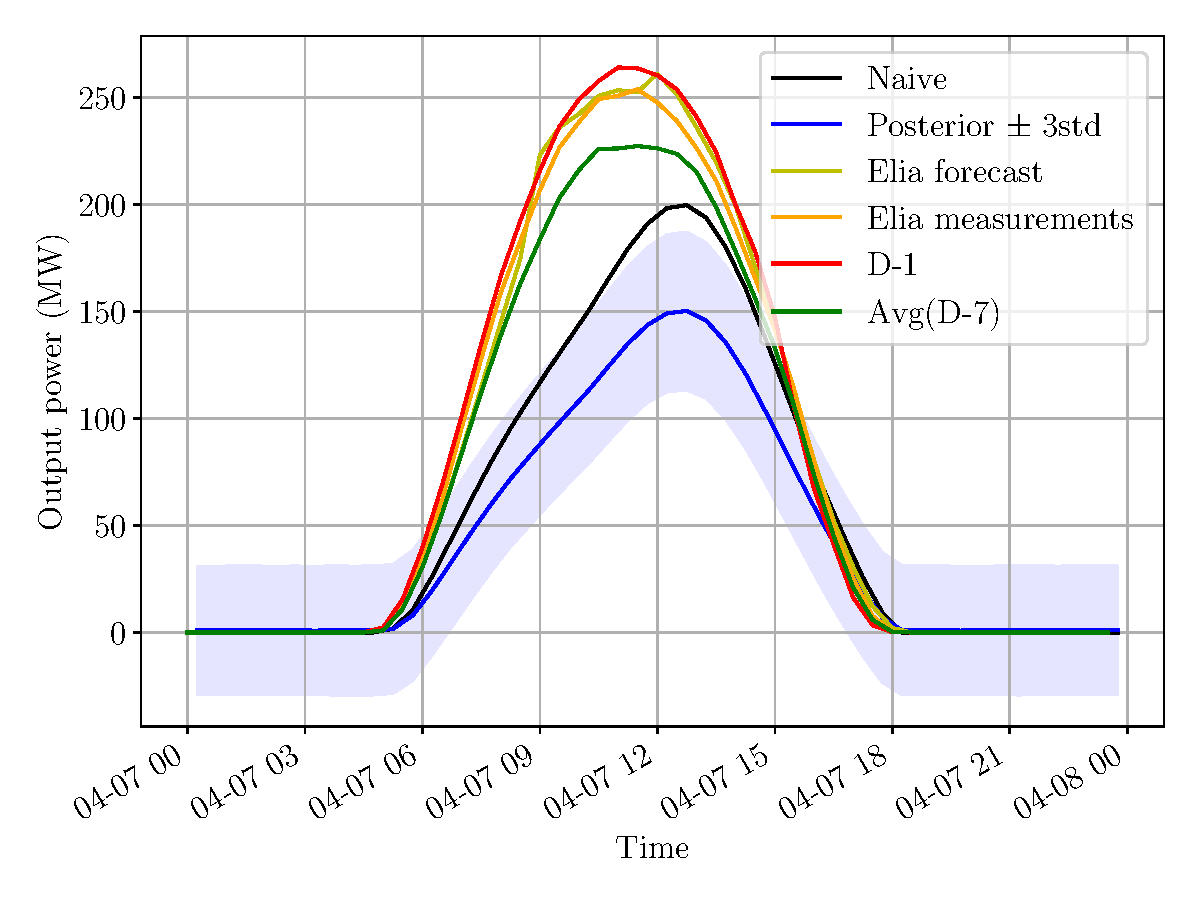
\includegraphics[width=\textwidth]{resources/pdf/solar_panelwise_START_FOR_07-04-2020.pdf}
		\noskipcaption{Panelwise model (using irradiance forecasts).}
	\end{subfigure}
	\hspace{0em}
	\begin{subfigure}{0.48\textwidth}
		\centering
		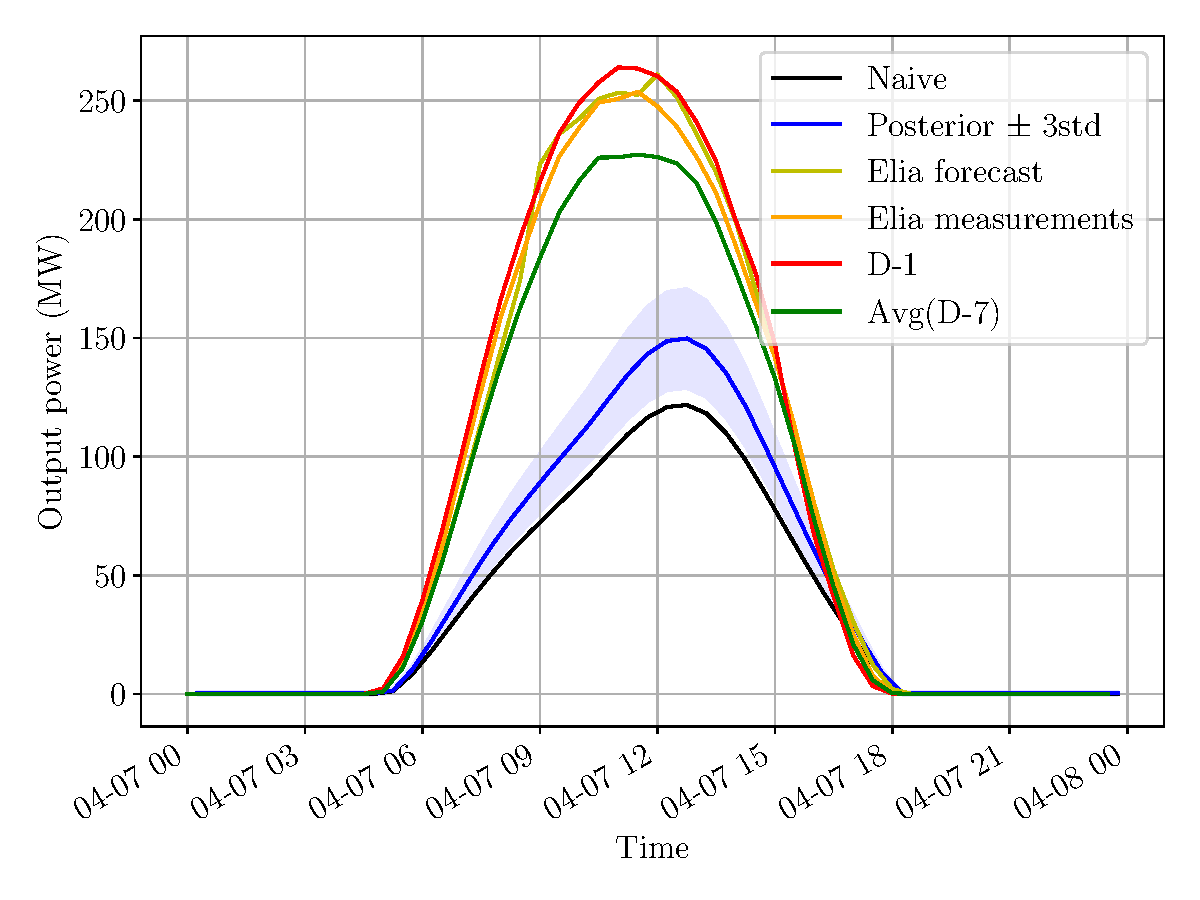
\includegraphics[width=\textwidth]{resources/pdf/solar_provincial_START_FOR_07-04-2020.pdf}
		\noskipcaption{Provincial model (using irradiance forecasts).}
	\end{subfigure}
\end{figure}
\end{frame}

\begin{frame}{Limitations}
    Although we obtain satisfactory results on average, some \alert{limitations} can be pointed out:
    \begin{itemize}
        \item \alert{Simplicity} of the models
        \item Using a \alert{single} source of irradiance data
        \item Strong \alert{influence} of the irradiance curve
        \item No real \alert{uncertainty} on our panels mapping
    \end{itemize}
\end{frame}

\begin{frame}{Limitations}
    \begin{figure}
    	\begin{subfigure}{0.48\textwidth}
		\centering
		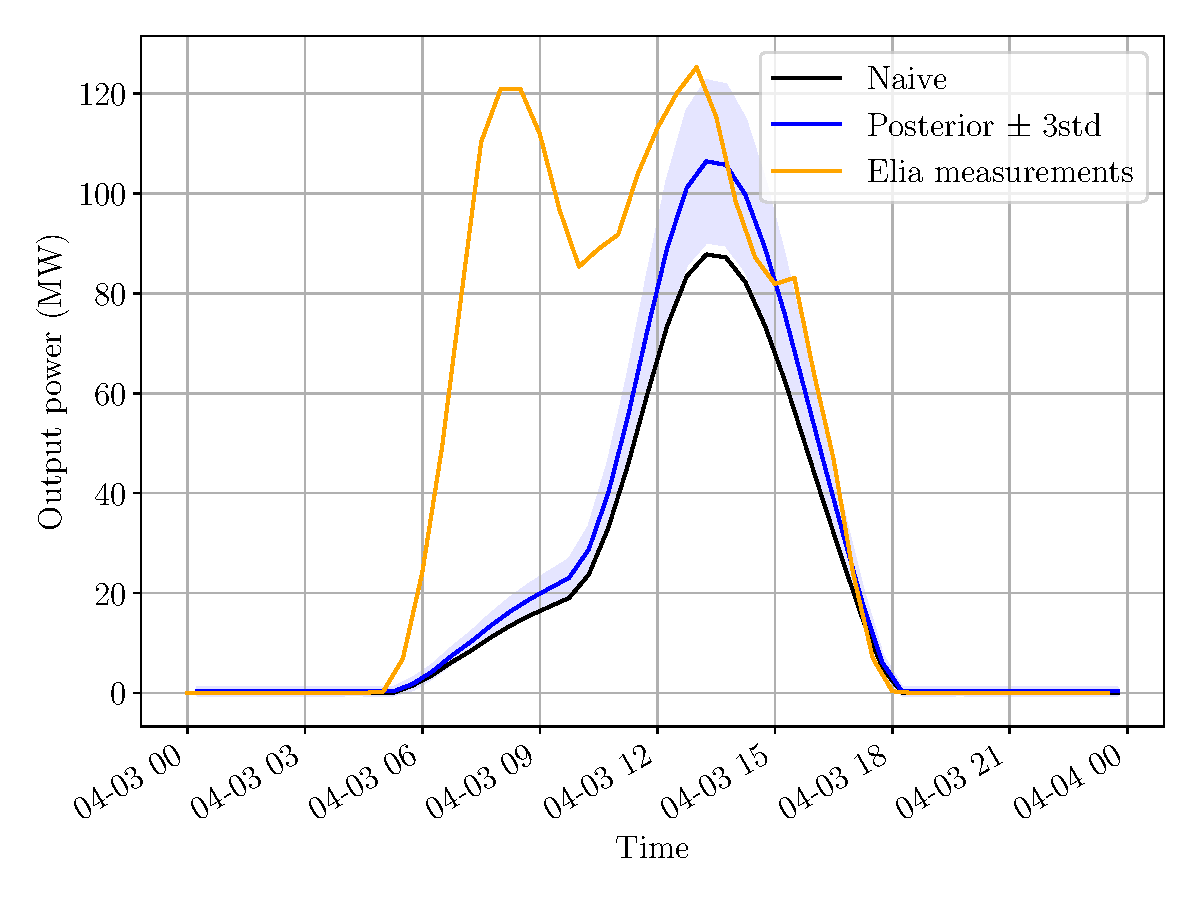
\includegraphics[width=\textwidth]{resources/pdf/solar_provincial_meas_for_START_FOR_03-04-2020.pdf}
		\caption{Provincial model.}
	\end{subfigure}
	\hspace{0em}
	\begin{subfigure}{0.48\textwidth}
		\centering
		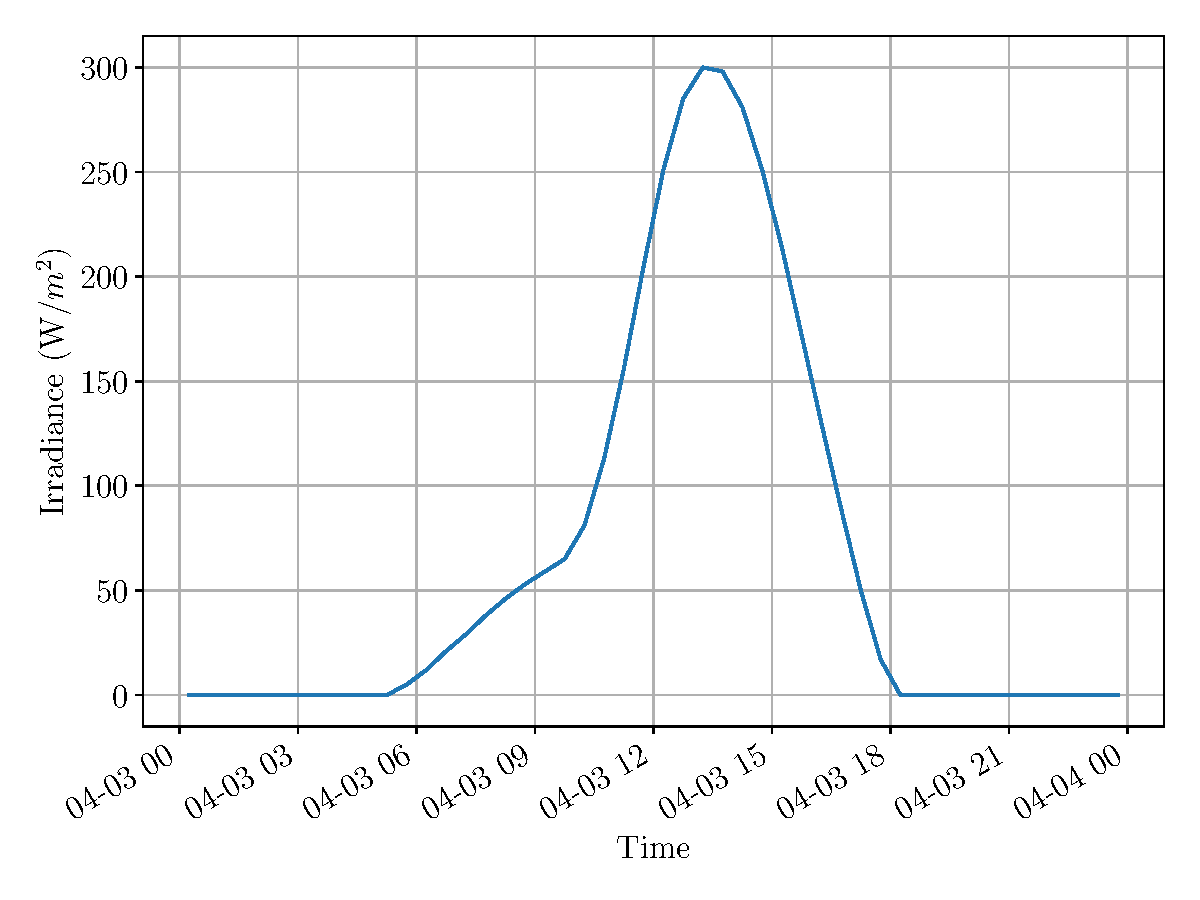
\includegraphics[width=\textwidth]{resources/pdf/irradiance_for_for_START_FOR_03-04-2020.pdf}
		\caption{Irradiance forecasted.}
	\end{subfigure}
\end{figure}
\end{frame}


\section{Wind power production}

\begin{frame}{Wind forecasting problem}
	Wind power forecasting \alert{problems classification}:
	\begin{itemize}
		\item Immediate-short-term (a few hour ahead);
		\item \alert<2>{Medium-term (few hours to several days)};
		\item Long-term (multiple days ahead).
	\end{itemize}
\end{frame}

\begin{frame}{Wind forecasting problem}
	Wind power forecasting \alert{approaches classification}
	\begin{itemize}
		\item \textbf{Physical modelling}: from physical parameters and NWP\footnote{Numerical Weather Prediction};
		\item \textbf{Statistical modelling}:
		\begin{itemize}
			\item \textbf{Time series forecasting}: from power time series;
			\item \alert<2>{\textbf{NWP post-processing}}: from NWP.
		\end{itemize}
		\item \textbf{Hybrid approaches}: various approaches (constrained regression, physical model as input feature, etc. \textit{e.g.} WPPT \parencite{croonenbroeck2014windpower}).
	\end{itemize}
\end{frame}

\begin{frame}{Physical model}
	\begin{figure}[H]
		\centering
		\begin{subfigure}[t]{0.48\textwidth}
			\centering
			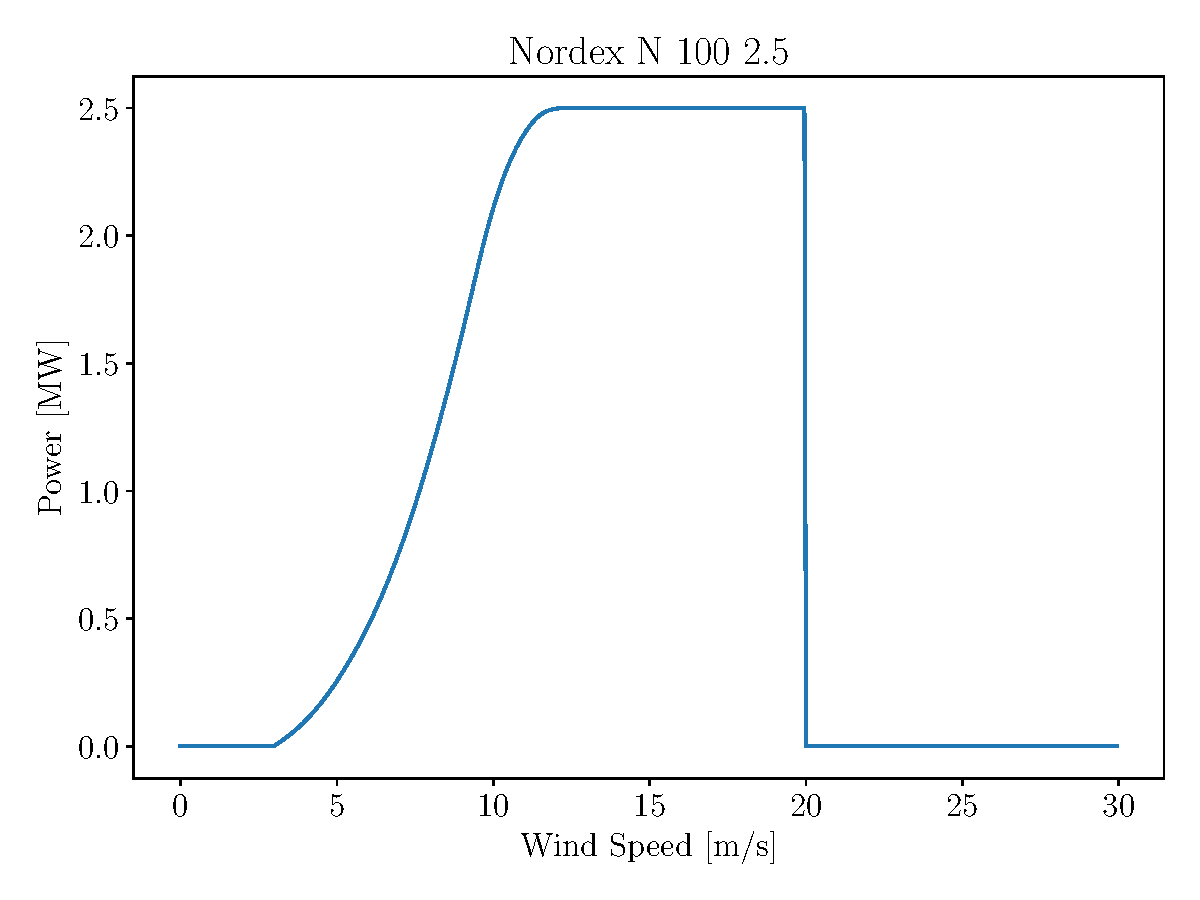
\includegraphics[width=\textwidth]{resources/pdf/wind_pc.pdf}
			\caption{Power curve}
		\end{subfigure}
		~ 
		\begin{subfigure}[t]{0.48\textwidth}
			\centering
			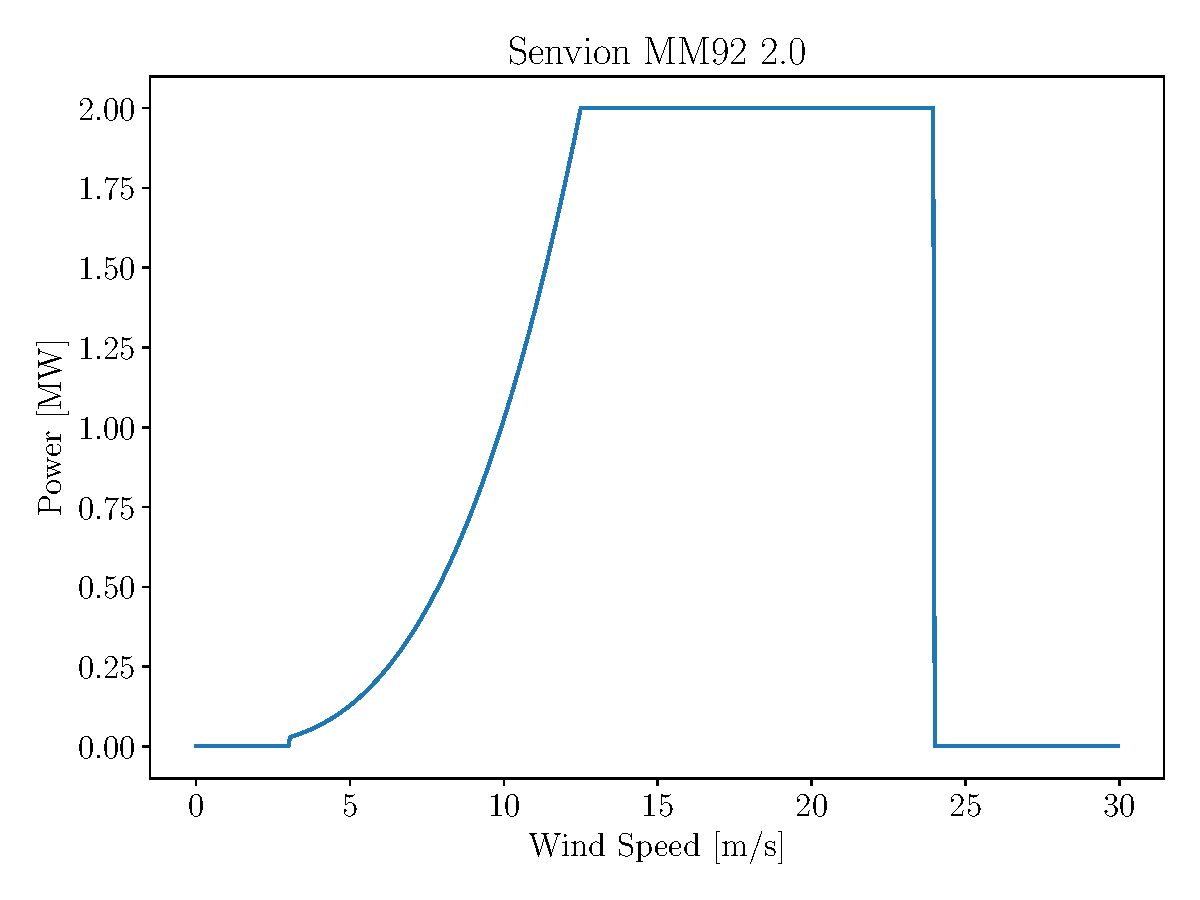
\includegraphics[width=\textwidth]{resources/pdf/wind_pc_theoretic.pdf}
			\caption{Theoretic power curve}
		\end{subfigure}
		\caption{Examples of power curves}
	\end{figure}
\end{frame}

\begin{frame}{Physical model}
	\begin{figure}[H]
		\centering
		\begin{subfigure}[t]{0.48\textwidth}
			\centering
			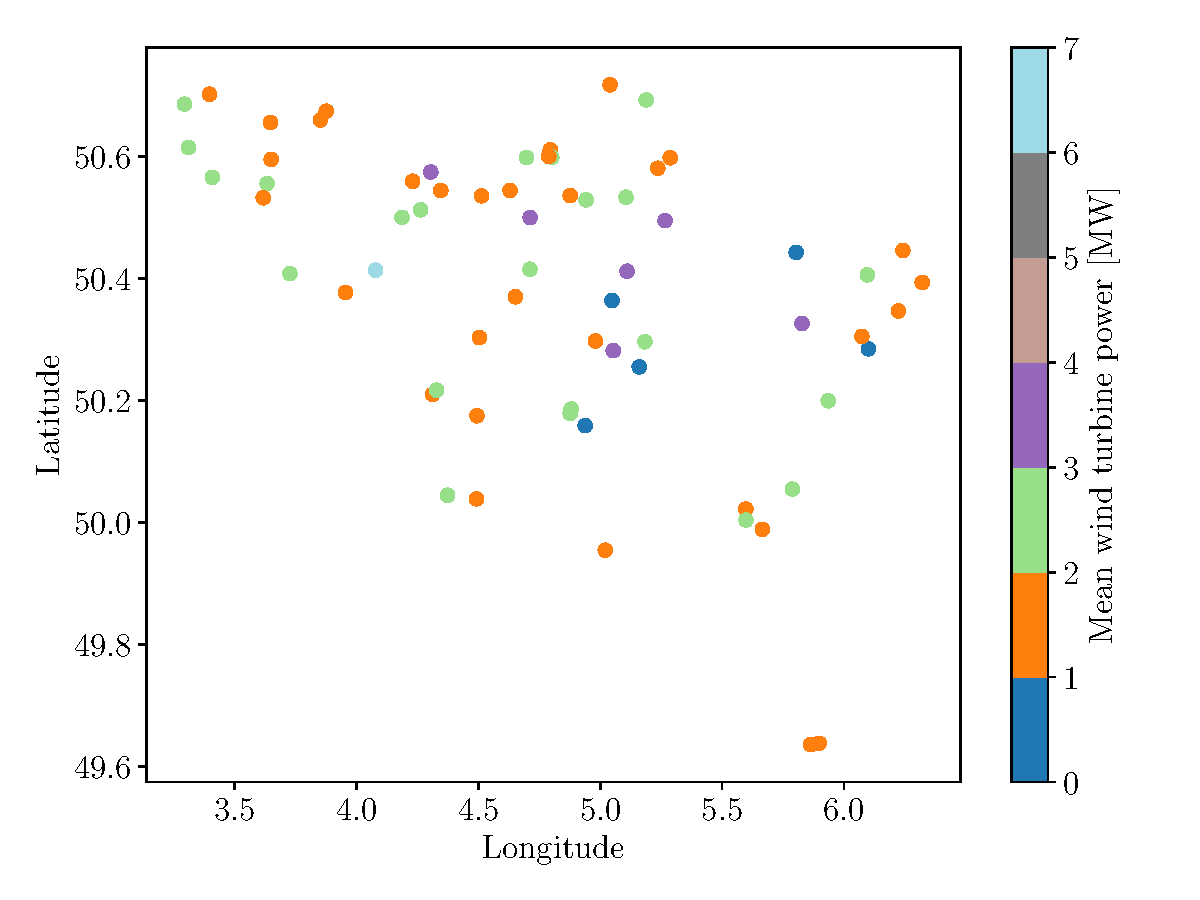
\includegraphics[width=\textwidth]{resources/pdf/wind_farms.pdf}
			\caption{Wind power plants in Wallonia}
		\end{subfigure}
		~
		\begin{subfigure}[t]{0.48\textwidth}
			\centering
			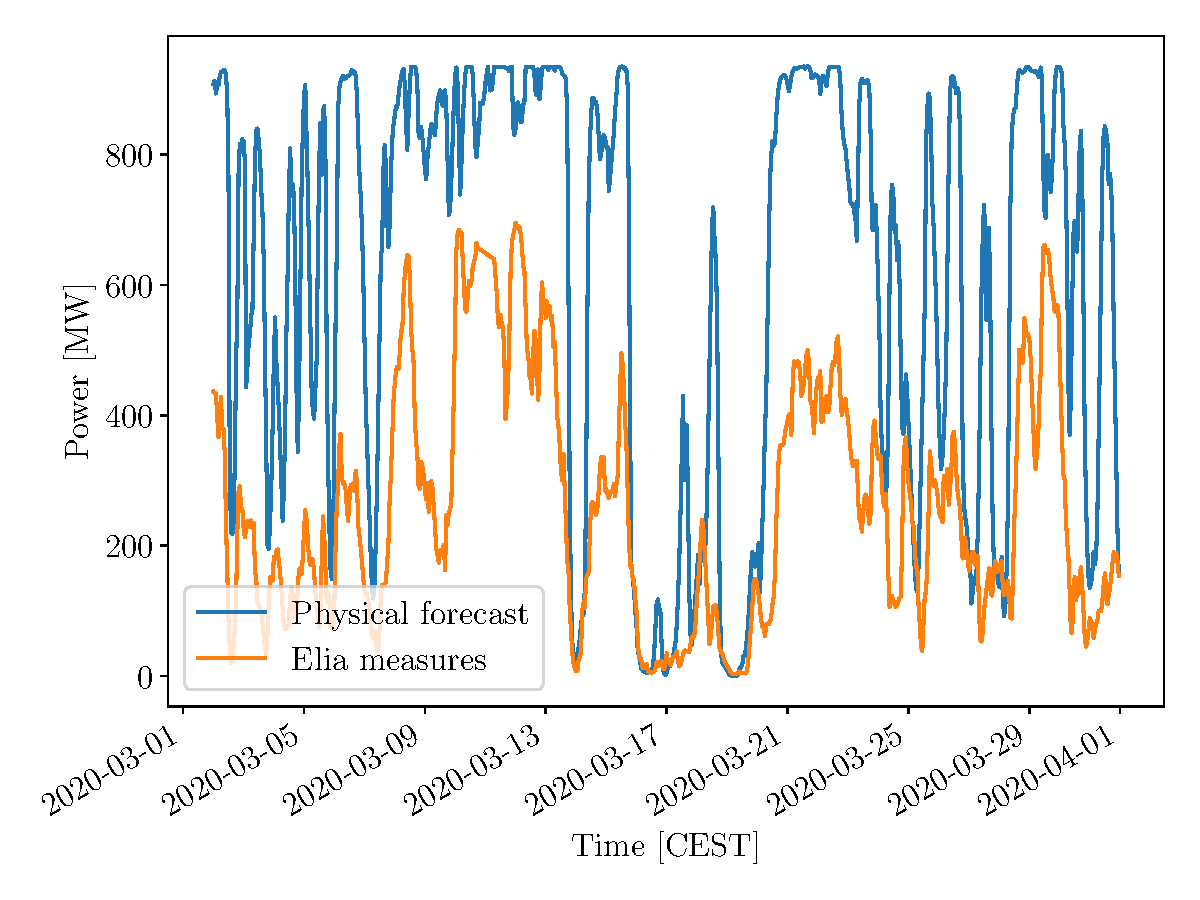
\includegraphics[width=\textwidth]{resources/pdf/wind_phys.pdf}
			\caption{Physical model forecast example}
		\end{subfigure}
		\caption{Wind power plants location and physical model}
	\end{figure}

	MAE: \SI{355.16}{\mega\watt} (maximum measured power of \SI{727}{\mega\watt})
\end{frame}

\begin{frame}{Data and computation flow}
	\begin{figure}
		\centering
		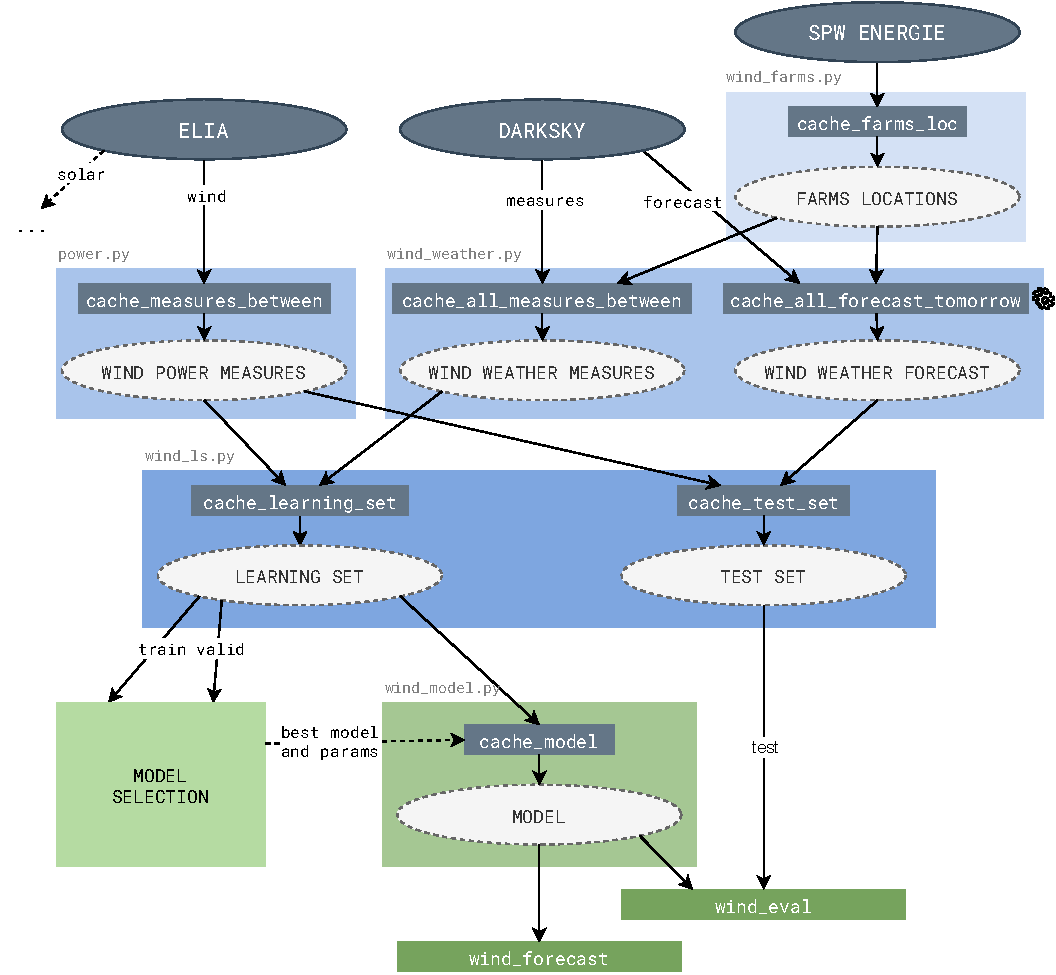
\includegraphics[width=.8\textwidth]{resources/pdf/diagram_wind.pdf}
	\end{figure}
\end{frame}

\begin{frame}{Feasibility of the regression}
	\begin{figure}[H]
		\centering
		\begin{subfigure}{.48\textwidth}
			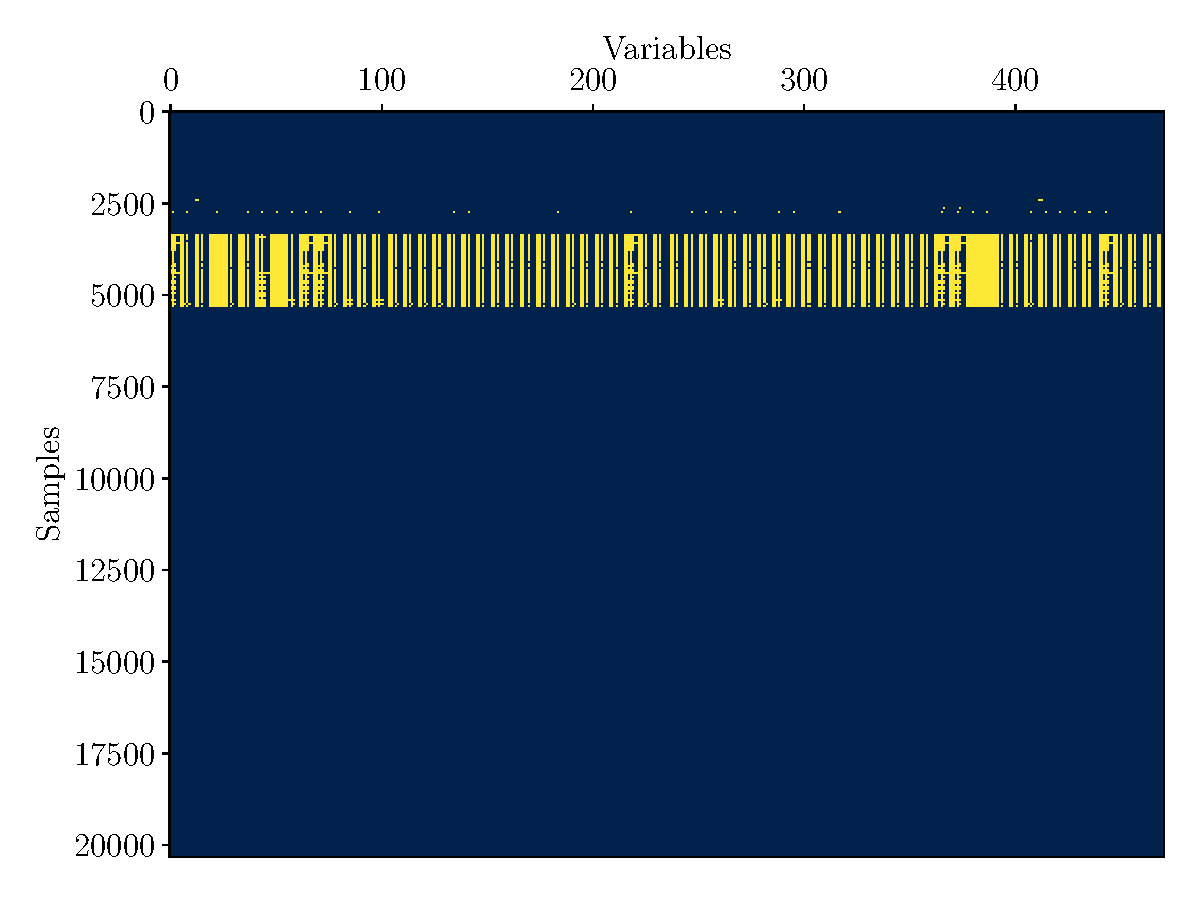
\includegraphics[width=\textwidth]{resources/pdf/wind_missingness.pdf}
			\caption{Missingness in the learning set (2069 NA corresponding to \SI{0.024}{\percent})}
		\end{subfigure}
		~
		\begin{subfigure}{.48\textwidth}
			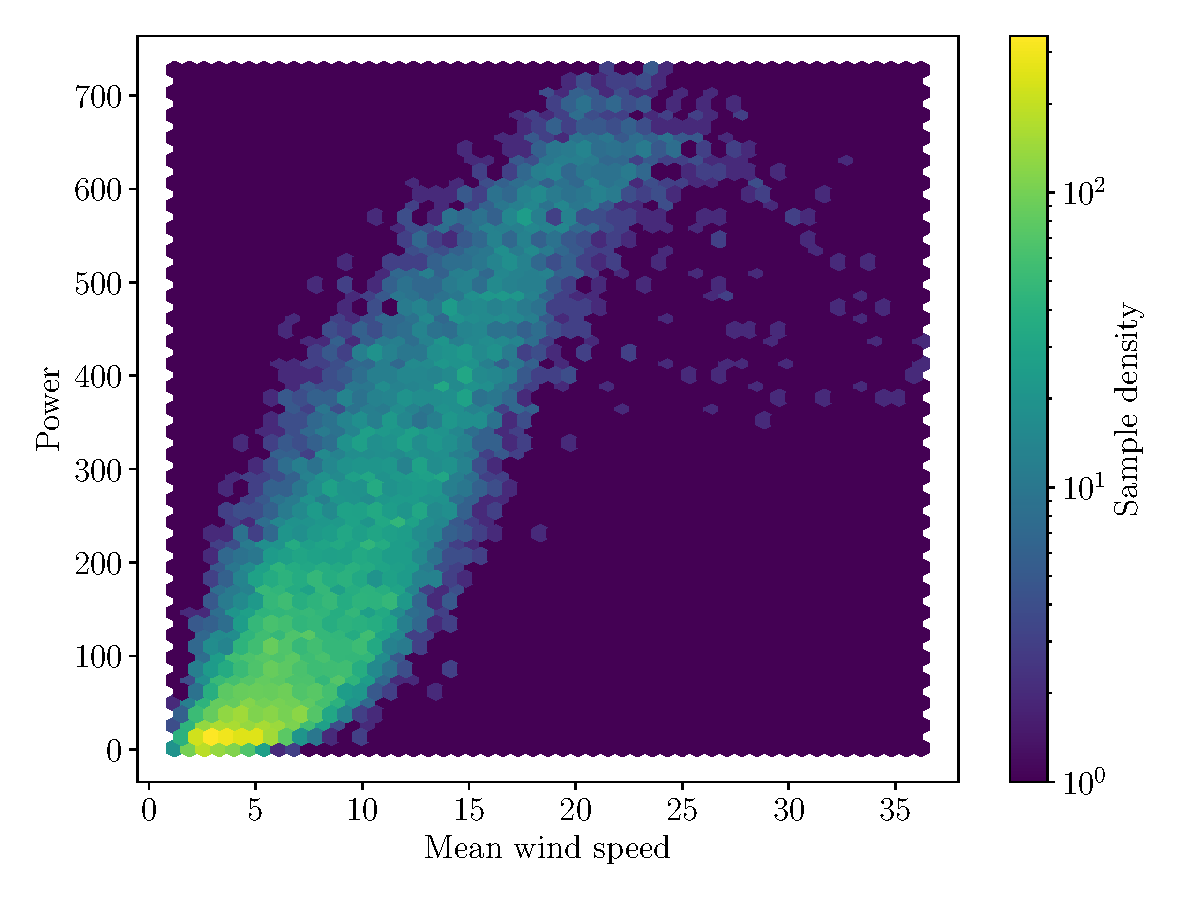
\includegraphics[width=\textwidth]{resources/pdf/wind_wallonia_pc.pdf}
			\caption{Learning set sample density with respect to the total power and the mean wind speed at the 67 wind power plants location}
		\end{subfigure}
	\end{figure}
\end{frame}

\begin{frame}{Feature selection}
	\begin{figure}
		\centering
		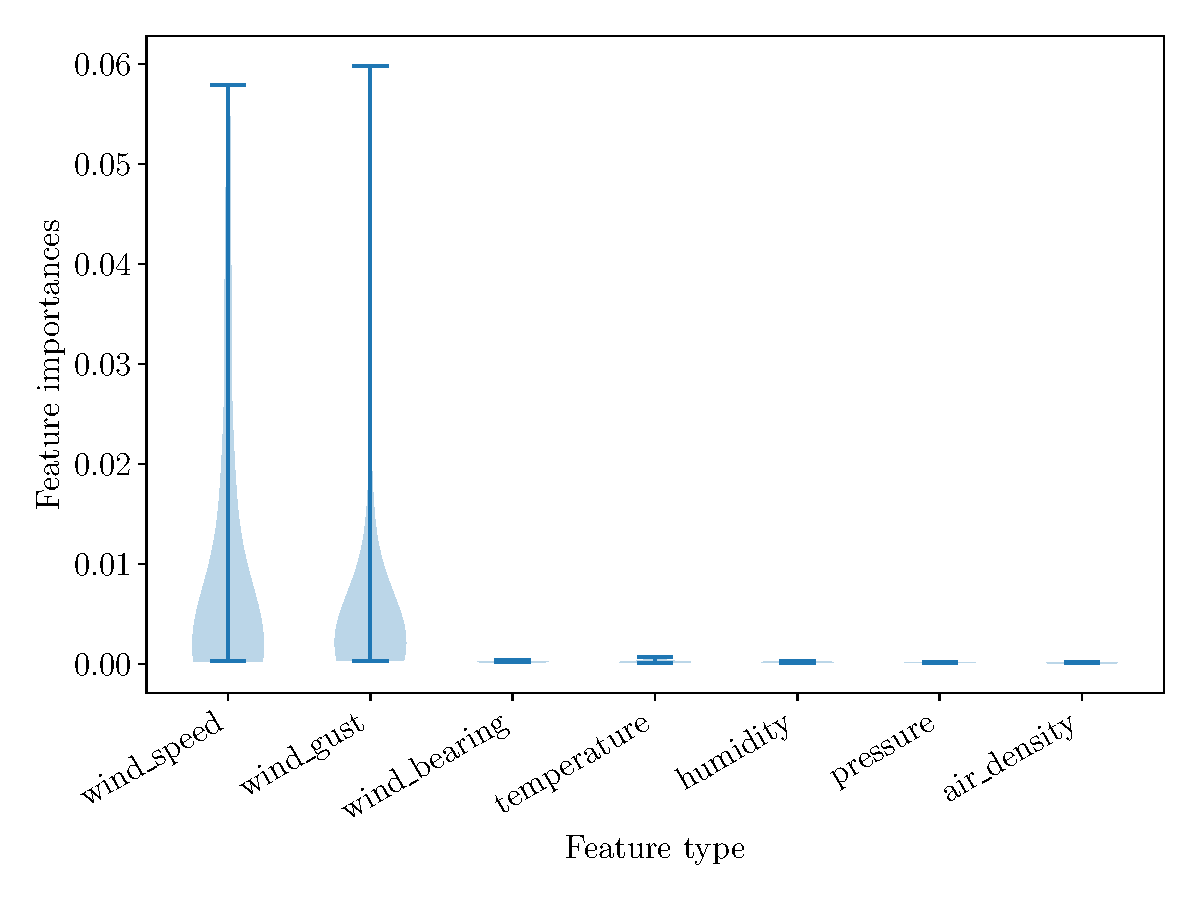
\includegraphics[width=0.8\textwidth]{resources/pdf/wind_fi.pdf}
		\vspace{-1em}
		\caption{Feature importances distribution with respect to the type of feature}
	\end{figure}
\end{frame}

\begin{frame}{Supervised learning methods}
	The following supervised learning methods have been extensively experimented
	\begin{itemize}
		\item \emph{Quantile} Extra Trees: variant of the extra trees where each leaf contains all learning samples that ended up in it, instead of only the mean. Quantiles estimated at prediction time.
		\item \emph{Quantile} Gradient Boosting: gradient boosting is performed on the quantile loss:
		\begin{equation*}
			\alpha(y, q) = \begin{cases}
				\abs{y - q} \alpha & \text{ if } y > q \\
				\abs{y - q} (1 - \alpha) & \text{ else }
			\end{cases}
		\end{equation*}
	\end{itemize}
\end{frame}

\begin{frame}{Hyper-parameters}
	Hyper-parameters have been slightly tuned to:
	\begin{itemize}
		\item \emph{Quantile Extra Trees}: \num{1000} estimators, minimum number of samples required to split: \num{10}, number of features to consider when looking for the best split: all.
		\item \emph{Quantile Gradient Boosting}: \num{1000} estimators, learning rate: \num{0.1}, number of features to consider when looking for the best split: all, subsample: \num{0.7}.
	\end{itemize}
\end{frame}

\begin{frame}{Metrics}
	\begin{itemize}
		\item MAE (mean absolute error);
		\item nMAE (normalized mean absolute error);
		\item nRMSE (normalized root mean squared error);
		\item MQL10 (mean quantile loss for \num{10}\textsuperscript{th} quantile);
		\item MQL90 (mean quantile loss for \num{90}\textsuperscript{th} quantile).
	\end{itemize}
\end{frame}

\begin{frame}{Test sets}
	\begin{itemize}
		\item Shuffled sample split (\SI{25}{\percent})
		\item Last \SI{25}{\percent} of the data ($\approx$ six months).
		\item \emph{Weather forecast} test set: weather forecast for day $D$ has been requested on day $D - 1$ at 11 o'clock. (only between April 5 and April 27, 2020) % This allows to assess the quality of our model in real conditions, where weather measures for the next day are obviously not available. Unfortunately, this test set is only constituted of weather forecast .
		\item \emph{Weather measures} test set: same period as the \emph{weather forecast} test set.
	\end{itemize}
\end{frame}

\begin{frame}[t]{Results}
	\begin{table}[t]
		\centering
		\resizebox{\textwidth}{!}{%
		\begin{tabular}{|l|l|c|c|c|c|c|c|}
		\hline
			\textbf{Test set} &
				\textbf{Method} &
					\textbf{MAE} &
					\textbf{nMAE} &
					\textbf{nRMSE} &
					\textbf{MQL10} &
					\textbf{MQL90} &
					\textbf{Time}\footnotemark[\value{footnote}] [\si{\second}] \\ \hline
			
			\multirow{2}{.3\textwidth}{Shuffled TS (\alert<2,4>{Elia MAE: 34.87})} &
				\only<1-2>{Extra Trees &
					\alert<2>{31.14} &
					\SI{4.28}{\percent} &
					\SI{5.97}{\percent} &
					53.65 &
					57.78 &
					\alert<7>{752} \\ \cline{2-8} &
				Gradient Boosting &
					\alert<2>{32.90} & \SI{4.52}{\percent} &
					\SI{5.99}{\percent} &
					52.54 &
					51.90 &
					\alert<7>{0}
				}\only<3->{Extra Trees &
						- &
						- &
						- &
						- &
						- &
						\alert<7>{752} \\ \cline{2-8} &
					Gradient Boosting &
						- &
						- &
						- &
						- &
						- &
						\alert<7>{0}
				}
			\\ \hline
			\multirow{2}{.3\textwidth}{Last 6 months (\alert<2>{Elia MAE: 40.16})} &
				Extra Trees &
					\alert<2,5>{40.43} &
					\SI{5.56}{\percent} &
					\alert<8>{\SI{7.45}{\percent}} &
					64.58 &
					55.58 &
					\alert<7>{710} \\ \cline{2-8} &
				Gradient Boosting &
					\alert<2>{41.91} &
					\SI{5.76}{\percent} &
					\alert<8>{\SI{7.69}{\percent}} &
					\alert<6>{59.25} &
					\alert<6>{44.58} &
					\alert<7>{0} \\ \hline

			\multirow{2}{.3\textwidth}{Weather forecast (\alert<4>{Elia MAE: 21.51})} &
				Extra Trees &
					36.86 &
					\SI{5.07}{\percent} &
					\alert<8>{\SI{7.51}{\percent}} &
					52.51 &
					52.71 &
					\alert<7>{95} \\ \cline{2-8} &
				Gradient Boosting &
					\alert<5>{35.71} &
					\SI{4.91}{\percent} &
					\alert<8>{\SI{7.05}{\percent}} &
					\alert<6>{51.33} &
					\alert<6>{47.14} &
					\alert<7>{0} \\ \hline

			\multirow{2}{.3\textwidth}{Weather measures (\alert<4>{Elia MAE: 21.51})} &
				Extra Trees &
					33.26 &
					\SI{4.57}{\percent} &
					\alert<8>{\SI{6.44}{\percent}} &
					55.66 &
					47.26 &
					\alert<7>{115} \\ \cline{2-8} &
				Gradient Boosting &
					\alert<5>{31.62} &
					\SI{4.35}{\percent} &
					\alert<8>{\SI{5.87}{\percent}} &
					56.18 &
					\alert<6>{41.77} &
					\alert<7>{0} \\ \hline
		\end{tabular}}
		\caption{Results of the two algorithms on the learning sets (MAE and MQL are expressed in \si{\mega\watt})}
	\end{table}
	\vspace{-1em}
	%\begin{itemize}
		%\item<2->
		\only<1>{NB: On LS + TS, train time are \SI{188}{\second} and \SI{995}{\second} respectively.}
		\only<2,3>{1. First test set is invalid: information leakage between train and test set due to temporal correlation}
		\only<4>{2. \emph{Weather forecast} test set isn't representative and certainly lead to optimistic results}
		\only<5>{3. Gradient Boosting and Extra Trees are equivalent in terms of MAE and RMSE;}
		\only<6>{4. Gradient Boosting outperforms in terms of mean quantile losses;}
		\only<7>{5. Considering train and prediction time, Gradient Boosting is profitable while we train less than twice a year;}
		\only<8>{6. nRMSE results are comparable to results obtained in the literature \parencite{croonenbroeck2014windpower}, but we are working on weather measures.}
	%\end{itemize}
\end{frame}

\begin{frame}{Results - Extra Trees}
	\begin{figure}
		\centering
		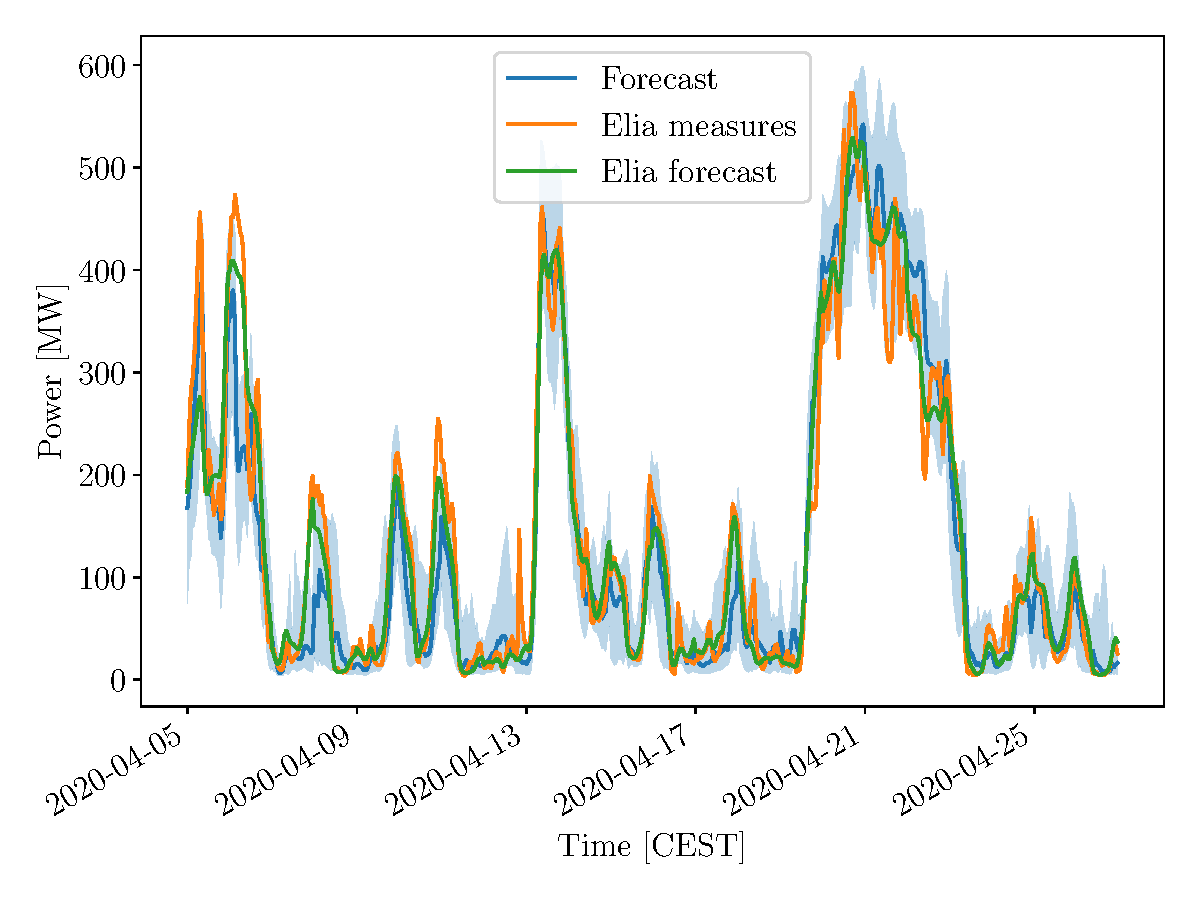
\includegraphics[width=.9\textwidth]{resources/pdf/wind_eval_qxt.pdf}
		\vspace{-1em}
		\caption{Quantile Extra Trees forecast}
	\end{figure}
\end{frame}

\begin{frame}{Results - Extra Trees}
	\begin{figure}
		\centering
		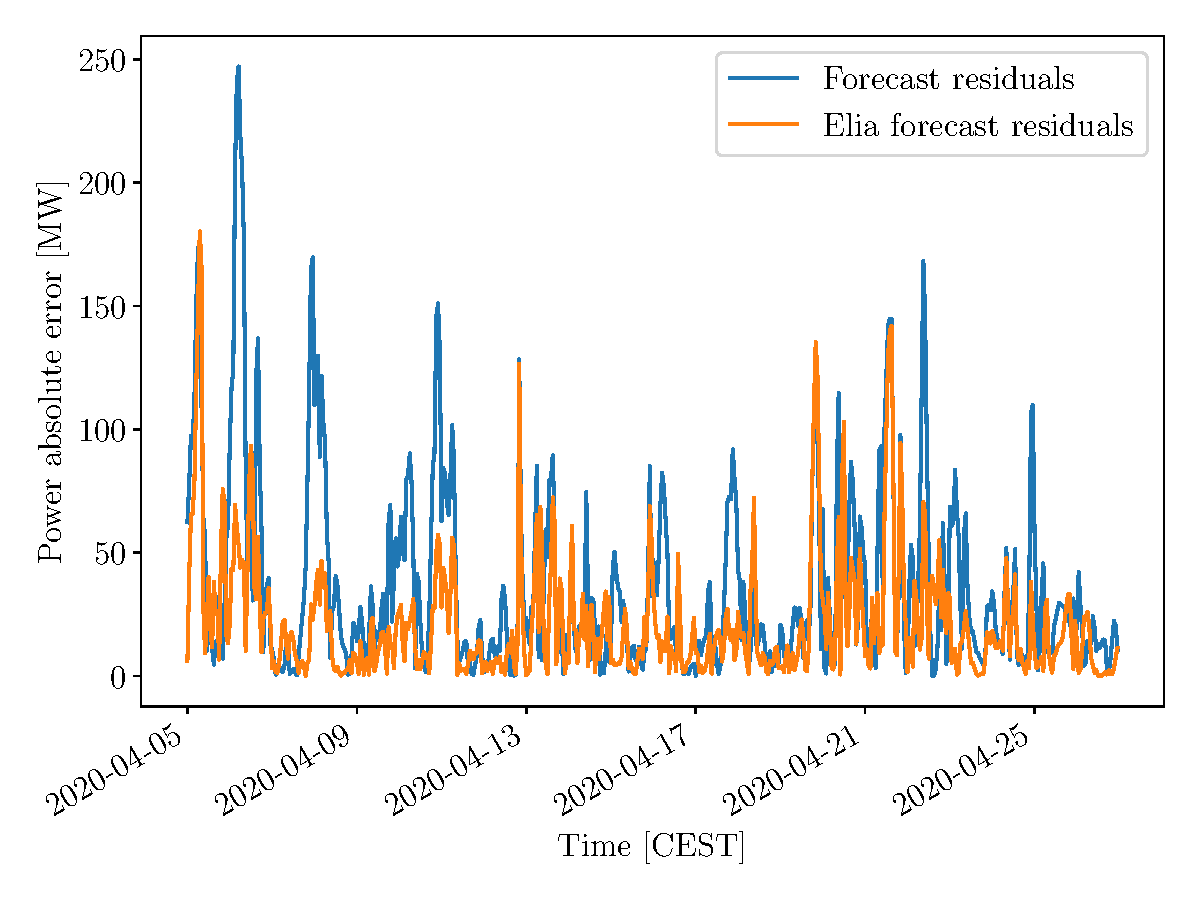
\includegraphics[width=.9\textwidth]{resources/pdf/wind_res_qxt.pdf}
		\vspace{-1em}
		\caption{Quantile Extra Trees forecast residuals}
	\end{figure}
\end{frame}

\begin{frame}{Limitations and improvements}
	\begin{itemize}
		\item Even if we can't assess the performance in real conditions (forecasting), we are certainly \alert{outperformed by Elia};
		\item We worked at the \alert{regional level} instead of provincial level, because of the \alert{unavailability of data}.
	\end{itemize}
	\begin{itemize}
		\item We could consider a \alert{hybrid approach} where we post process the output of the physical model (with or without NWP);
		\item  We could consider a hybrid approach that mix the \alert{two statistical approaches}: taking the temporal correlation into account to predict, even on the day-ahead task;
		\item Considering \alert{more complex} or fine-tuned \alert{SL models}, especially in the case of a time-series hybrid approach.
	\end{itemize}
\end{frame}

\section{Conclusion}

\begin{frame}{Conclusion}
	\begin{itemize}
	    \item We may regret the \alert{unavailability of data};
	    \item \alert{No past weather forecast} (wind or solar) is available, preventing us from assessing our models;
	    \item The photovoltaic power mapping has yielded very \alert{good accuracy} compared to the literature;
	    \item The photovoltaic mapping was \alert{able to adapt} to Belgian satellite imagery;
	    \item Solar and wind models \alert{perform as well as Elia} when based \alert{on weather measures} instead of weather forecasts;
	    \item Further \alert{improvements should be possible} for the three parts, if more data was available.
	\end{itemize}
\end{frame}

\begin{frame}[standout]
    \vspace{1em}
    Demonstration \\
    \href{https://znkvzr.com/apps/big-data/}{znkvzr.com/apps/big-data}
\end{frame}

\begin{frame}[allowframebreaks]
    \printbibliography
\end{frame}

\end{document}
